%=================================================================
%				preamble
%=================================================================
\documentclass[11pt,letterpaper]{book}

\newcommand{\theauthor}{Thomas Graf}		        
\newcommand{\university}{Stony Brook University}	
\newcommand{\emailaddress}{lin637@thomasgraf.net}
\newcommand{\coursenumber}{Lin637}
\newcommand{\coursename}{Computational Linguistics 2}
\newcommand{\thetitle}{\texorpdfstring{\coursenumber\\ \coursename}{\coursenumber --- \coursename}}
\newcommand{\thekeywords}{graduate level, lecture, computational linguistics, phonology, syntax}
\newcommand{\thedate}{}

\usepackage{mypackages}
\usepackage{mycommands}



%=================================================================
%			title format
%=================================================================
\author{\theauthor}
\title{\thetitle}
\date{\thedate}

%=================================================================
%			content
%=================================================================
% \includeonly{./tex/ConstituencyTests}

\begin{document}
\raggedbottom
\pagenumbering{Roman}
\maketitle
\tableofcontents
\clearpage

\setcounter{chapter}{-1}
\chapter{Syllabus --- You Better Read it!}
\label{cha:syllabus}
\setcounter{page}{1}
\pagestyle{fancy}

\fcolorbox{gray!25}{gray!25}{%
    \centering
    \begin{tabular}{ll}
        \textbf{Course:} Computational Linguistics 2\quad\qquad\qquad&
        \textbf{Name:} Thomas Graf\\
        \textbf{Course\#:} Lin637 &
        \textbf{Email:} lin637@thomasgraf.net\\
        \textbf{Time:} TR 10:00--11:20am &
        \textbf{Office hours:} Tue 11:30--2:30pm\\
        \textbf{Location:} tba & %fixme
        \textbf{Office:} SBS N249\\
        \textbf{Course Website:} tba & %fixme
        \textbf{Personal Website:} \url{http://thomasgraf.net}
    \end{tabular}
}

\section{What This Course is About}

\rotatebox{0}{
    \footnotesize
    \begin{tikzpicture}[
    every node/.style = { draw, thick },
    every path/.style = { ->, thick },
    sug/.style = { dashed },
    req/.style = { },
    ]
    \node[fill=gray!25] (CL2) at (0,0) [align=center] {Computational Linguistics 2\\ (Lin 637)};

    % Prereqs
    \node (Phon) [above=of CL2, xshift=-8em, align=center] {Phonology 1 (Lin 522)\\
                                                                \emph{or}\\
                                                            Phonetics (Lin 523)
                                                        };
    \node (Syntax) [left=of Phon, align=center] {Syntax 1\\ (Lin 521)};
    \node (Math)   [above=of CL2, xshift=8em, align=center] {Statistics (Lin 538)\\
                                                                \emph{or}\\
                                                            Mathematical Methods (Lin 539)
                                                        };
    \node (CL1) [right=of Math, align=center] {CompLing 1\\ (Lin 537)};

    % CS branch
    \node (NLP) [below right=of CL2, xshift= 8em, align=center] {Introduction to NLP\\ (CSE 628)};
    \node (Machine) [below=of NLP, xshift=-8em, align=center]  {Machine Learning\\ (CSE 512)};
    \node (Speech)  [below=of NLP, xshift= 8em, align=center] {Speech Processing\\ (CSE 542)};
    \node (AI) [below=of Machine, align=center] {Artificial Intelligence\\ (CSE 537)};

    % Linguistics branch
    \node (CompSem) [below=of CL2, xshift=-16em, align=center] {Computational Semantics\\ (Lin 626)};
    \node (CompPhon) [below=of CompSem, align=center] {Computational Phonology\\ (Lin 627)};
    \node (CompSyn) [below=of CompPhon, align=center] {Computational Syntax\\ (Lin 628)};

    \node (Learn) [right=of CompSem, xshift=4em, align=center]  {Learnability\\ (Lin 629)};
    \node (Parse) [right=of CompPhon, xshift=4em, align=center] {Parsing and Processing\\ (Lin 630)};

    % Branches
    \draw[sug] (Syntax) |- (CL2);
    \draw[sug] (Phon) to (CL2);
    \draw[sug] (Math) to (CL2);
    \draw[req] (CL1) |- (CL2);
    \draw[req] (CL1.south -| NLP.north) -- (NLP);
    \draw[sug] (NLP) -| (Machine);
    \draw[sug] (NLP) -| (Speech);
    \draw[sug] (NLP) |- (AI);
    \draw[sug] (Learn |- CL2.south) -- (Learn); 
    \draw[sug, transform canvas={xshift=2em}] (Parse |- CL2.south) -- (Parse);
    \draw[sug] ($(CL2.south)-(6em,0)$) |- (CompSem);
    \draw[sug] ($(CL2.south)-(5em,0)$) |- (CompPhon);
    \draw[sug] ($(CL2.south)-(4em,0)$) |- (CompSyn);
\end{tikzpicture}

}

\begin{table}
    \centering
    \begin{tabular}{rlp{4.5cm}p{4.5cm}p{4cm}}
        \hline
        \hline
        \emph{Wk} & \emph{Classes} & \emph{Formal} & \emph{Linguistics} & \emph{Algorithms}\\\hline
        1         & Jan 27, 29     & What is computation? & History\\
        2         & Feb 3, 5       & Formalizing phonology & Why formalize?\\
        3         & Feb 10, 12     & Strictly local languages & Local dependencies\\
        4         & Feb 17, 19     & Subregular hierarchy & How powerful is phonology?\\
        5         & Feb 24, 26     & Regular languages & Abstractness\\
        6         & (DGFS)         & & \\
        7         & Mar 10, 12     & String transductions & SPE-OT equivalence\\
        \hline                       
        8         & (Spring Break) & & \\
        \hline                       
        9         & Mar 24, 26     & Weak Generative Capacity & $\text{Phonology} < \text{Syntax}$\\
        10        & Mar 31, Apr 2  & Tree languages & \\
        11        & Apr 7, 9       & Local tree languages & \\
        12        & (GLOW)         & & \\
        13        & Apr 21, 23     & Recognizable tree languages & \\
        14        & Apr 28, 30     & TAG and MGs & \\
        15        & May 5, 7       & Tree transductions & Reinterpreting the T-model\\
        \hline
        \hline
    \end{tabular}
\caption{Tentative course outline}
\end{table}


\section{Teaching Goals}
\begin{itemize}
    \item \textbf{General Skills}
        \begin{itemize}
            \item construct a logically sound argument
            \item evaluate the predictions and implications of an argument with respect to a given set of data
            \item compare and weigh different arguments
            \item knowledge of common logical fallacies and unsound reasoning steps
            \item disprove an empirically wrong or logically flawed argument 
            \item ability to detect and succinctly describe patterns in a given data sample
            \item understand the interplay of data and theory in the sciences
        \end{itemize}
    \item \textbf{Linguistic Skills}
        \begin{itemize}
            \item knowledge of a wide range of parts of speech
            \item familiarity with phrase structure rules
            \item writing phrase structure grammars to account for a given phenomenon
            \item lexicalizing rules
            \item a general understanding why computers still fail miserably at linguistic tasks
        \end{itemize}
    \item \textbf{What is it good for?}
        \begin{itemize}
            \item Argumentation and reasoning skills are the most important skill out there.
                People try to trick you all the time --- reasoning skills are your primary means of intellectual self-defense.
            \item Phrase structure grammars are widely used in the IT industry, e.g.\ by \emph{Xerox}, \emph{Nuance}, \emph{IBM} and \emph{Google}.
            \item Writing good grammars is difficult and an important skill in the construction of tree banks (text corpora where each sentence is annotated with syntactic structure). Tree banks are an essential tool for all areas of natural language processing by computers, e.g.\ machine translation, text generation and summarization, dialog systems and so on.
            \item Familiarity with syntactic structure and dependencies makes learning new languages easier.
        \end{itemize}
\end{itemize}


\section{Grading}
\begin{itemize}
    \item \textbf{Homework}\\
        weekly exercises and/or programming assignments; a random sample of homeworks will be collected and graded; solutions will be made available online after the due date
    \item \textbf{Readings}\\
        assigned on a weekly basis; you have to collectively write a summary for each reading in the course wiki (remember, it's a wiki, so everyone can tell from the editing history how much you contributed) 
    \item \textbf{Lecture Evaluations}\\
    \item \textbf{Presentation}\\
        everyone has to pick a research topic and present it at a workshop during finals week
\end{itemize}


\section{Policies}

\subsection{Contacting me}
\begin{itemize}
    \item Emails should be sent to lin637@thomasgraf.net to make sure they go to my high priority inbox.
        Disregarding this policy means late replies and is a sure-fire way to get on my bad side.
    \item Reply time < 24h in simple cases, possibly more if meddling with bureaucracy is involved.
    \item If you want to come to my office hours and anticipate a longer meeting, please email me so that we can set apart enough time and avoid collisions with other students.
\end{itemize}

\subsection{Attendance}
\begin{itemize}
    \item You do not have to show up for the lecture. However, asking questions and participating in discussions during class will improve your grade.
    \item Handouts and homeworks are posted on Blackboard.
\end{itemize}

\subsection{Homework}
\begin{itemize}
    \item Weekly homeworks, posted on Blackboard every Wednesday by 11:59pm
    \item Due the following Wednesday by 7pm (student office drop-off box)
    \item No late hand-ins!
    \item Homeworks must be typed up and printed!
    \item Collaboration on homework problems is encouraged as long as you write up the solutions by yourself, using your own words and examples.
        Most homework exercises will be fairly open ended, so it will be easy for us to see if you simply copied somebody's answer.
        Copying another student's solutions is considered cheating, with all the unpleasant consequences this entails.
\end{itemize}

\subsection{Special Needs \& Retaking the Course}
\begin{itemize}
    \item If you have any special needs that might impact your class performance (learning disabilities, impaired sight or hearing, etc.), please come to my office hours or contact me via mail so we can make suitable arrangements.
    \item If you already know that you'll be missing recitation or an exam due to religious holidays or other binding commitments, please send me an email with the specific dates.
    \item If you've taken this course before, I invite you to come to my office hours this week so we can identify problem areas and discuss how to address them.
\end{itemize}

\section{How to Ace This Course}

\begin{itemize}
    \item \textbf{Do the homeworks!}\\
        Do every single homework.
        Each homework is about 5\% of your grade.
        %
    \item \textbf{Chase those bonus points!}\\
        Try the challenge exercises, even if you aren't quite sure what the answer is.
        You might still get some points, and wrong answers aren't penalized.
        Similarly, take every single quiz to minimize the risk of a bad final dragging down your grade.
        %
    \item \textbf{Don't rush into things!}\\
        Read every question carefully (this goes for homeworks as well as quizzes).
        Make sure you know what it is you are asked to do.
        Whenever you feel like starting the solution, stop for a moment, paraphrase the question you think you are answering, and double check that this is indeed what the exercise is asking.
        %
    \item \textbf{Reflect on what you are doing!}\\
        Think about why certain exercises are on the homework.
        We're not trying to torture you, there is a reason for every single exercise, some important insight waiting to be discovered by you.
        Rote memorization is not enough for this course, you must understand the tools and how to use them.
        %
    \item \textbf{Collaborate!}\\
        Don't be a lone wolf, discuss the homework with your peers.
        That way, you make sure that you aren't misinterpreting the question, and by explaining your answer to others you can see whether it actually works, and why.
        But don't just copy somebody's answers.
        %
    \item \textbf{Ask for help before it's too late!}\\
        If you feel that you're falling behind, act immediately.
        Go to your TAs or come to my office hours so that we can go over the material you are struggling with.
        This is not like an introductory survey course where you can skip a session and start fresh on a new topic the week after that.
        Everything builds on the material that came before.
        Treat it like learning a foreign language, programming or calculus.
        Any knowledge gaps you have will grow at a rapid pace if you don't act fast.
\end{itemize}

\medskip
\begin{flushright}
    \begin{minipage}[b]{28em}
        \flushright
        \emph{The mind is not a vessel to be filled but a fire to be kindled.}\\
        Plutarch\\

        \medskip
        \emph{Learning is exploring.}\\
        Yours truly
    \end{minipage}
\end{flushright}

\pagenumbering{arabic}

\chapter{Implementing Phonology as a List}
\label{cha:ListPhonology}

Linguists distinguish many different aspects of language:
%
\begin{description}
    \item[Phonetics]
        the physical properties or speech, in particular the physiological production of sounds (\emph{articulatory phonetics}) and their acoustic properties (\emph{acoustic phonetics})
    \item[Phonology]
        the rules regulating the sounds of a language: which sounds are part of a given language's inventory, in which positions may they occur, how are sounds affected by the presence of other sounds, which syllables in a word are stressed, and so on
    \item[Morphology]
        the rules regulating the structure of words, in particular how a words form can change depending on certain features such as person or number (\emph{inflectional morphology}) and how new words can be built from other words (\emph{derivational morphology})
    \item[Syntax]
        the rules regulating the structure of sentences, e.g.\ word order and morphosyntactic dependencies (person, gender, number agreement)
    \item[Semantics]
        the formal study of the meaning of words (\emph{lexical semantics}) and how the logical meaning of a sentence is derived from the meaning of its words (\emph{compositional semantics})
    \item[Pragmatics]
        the study of how a sentence's intended meaning arises from the interaction of its logical meaning and the discourse context
\end{description}

All these areas have been looked at by computational linguists, but we will start with phonology, for several reasons.
First, phonetics involves a lot of non-discrete math that is fairly demanding for the uninitiated.
Similarly, syntax, semantics and pragmatics use fairly complicated linguistic formalisms.
This leaves us with phonology and morphology, and since the two are very similar from a computational perspective (many computational models even handle them both at the same time), we pick the one that linguistics students usually have had greater exposure to: phonology.

\section{A Simple Phonology Problem}

Word-final devoicing is a process that has been extensively studied by phonologists.
As its name implies, final devoicing turns voiced consonants (\textipa{/b/}, \textipa{/d/}, \textipa{/g/}, \textipa{/z/}, \ldots) that occur at the end of a word into their voiceless counterparts (\textipa{/p/}, \textipa{/t/}, \textipa{/k/}, \textipa{/s/}, \ldots).
It usually applies only to a proper subclass of a given language's full inventory of voiced sounds.
Final devoicing is attested in a rich variety of languages, from Indo-European ones like Catalan (Romance), German (Germanic), and Russian (Slavic) to Turkish (Turkic, Altaic) and Wolof (Senegambian, Niger-Congo).

\begin{center}
    \begin{tabular}{r@{\hskip 4em}ll}
        \toprule
        \textbf{Language} & \textbf{Voiced} & \textbf{Devoiced}\\
        \toprule
        Catalan & \emph{grize} `gray (\gloss{f})' & \emph{gris} `gray (\gloss{m})'\\
        German & \emph{räder} `bikes' & \emph{rat} `bike'\\
        Russian & \emph{kniga} `book (\gloss{Nom.Sg.}) & \emph{knik} `book (\gloss{Gen.Pl.})'\\
        Turkish & \emph{sarabi} `wine (\gloss{Acc.Sg.})' & \emph{sarap} `wine (\gloss{Nom.Sg.})'\\
        Wolof &  does anybody know & the data?\\
        \bottomrule
    \end{tabular}
\end{center}

What kind of computational resources must a native speaker possess that has successfully learned this process for their language and can apply it correctly during speech?
As innocent as this question may seem, it is actually very difficult to answer because it is unclear what kind of computational process underlies word-final devoicing.

The way it was described above --- which is the standard view among phonologists --- it is a process that takes a word as an input and returns an output where any word-final voiced consonants have been devoiced.
That is a complex idea that involves three distinct components:
%
\begin{enumerate*}
    \item an input form,
    \item an output form,
    \item a process translating the former into the latter.
\end{enumerate*}
%
It is far from obvious that this is indeed what speakers are doing; all we can tell for sure is that speakers produce the correct output forms.
So rather than jumping immediately into the deep waters of sophisticated phonological machinery, let's see what the \textbf{simplest empirically adequate} solution might be.
It might well turn out that speakers are actually doing something more complicated, but at least we will have a better understanding of the problem and a computational baseline that we can compare speakers' behavior to.

Arguably the simplest conceivable solution is that there are no phonological processes at all, speakers simply memorize all the output forms.
%
\begin{description}
    \item[List Phonology Model] A speaker's knowledge of phonology is fully captured by a list of pronunciations.
\end{description}
%
This would reduce phonology to a long list of fully inflected words and speakers simply pick that item from the list that they want to pronounce.
It explains speakers' ability to produce the correct output form purely via memorization, no computational machinery is required beyond a mechanism for storing and retrieving phonetic strings. 
Such a solution is certainly simple, and it has been used in NLP in the past.
After all it only require a few people to go through a dictionary of English and write down the pronunciation for each word and all its fully inflected variants (e.g.\ \emph{go}, \emph{goes}, \emph{went}, \emph{gone}, \emph{going}).
Simple as it may be, though, the important question for us whether it is empirically adequate.

\section{Storage and Retrieval Speed}

\subsection{Lists, Hash Tables, and Python Dictionaries}

Let's first think about whether speakers could possibly have such a list stored somewhere in their brain.
Psychologists and neuroscientists still know very little about how the brain stores information, so for the sake of argument we will look at this through the lens of Python data structures.
Python has lists as a data type, so we could instantiate a phonology list for a given language, say German.
%
\Note{This list uses the \href{http://www.kirshenbaum.net/IPA/ascii-ipa.pdf}{sci.lang ASCII transliteration} of IPA, which is easier to type and can be used on systems without unicode support.}
\begin{center}
    \begin{pythoncode}
        german_phonology = ['Ra:t', 'Re:dV"', 'blint', 'blind@',\
                            'iC', 'du:', 'EV"', 'si:', 'Es']
    \end{pythoncode}
\end{center}
%
The problem is that items in a list are not always easy to retrieve.
If you know the index of an item, you can immediately access it via said index.
%
\begin{center}
    \begin{pythoncode}
        german_phonology[4]
    \end{pythoncode}
\end{center}
%
But with long lists you do not know which position a specific item occupies.
In order to retrieve this item, then, one has to search through the entire list until one finds the correct item.
So the longer the list, the longer it takes to find an item towards its end.
If we simply search through the list from left to right, finding the $n$-th item takes $n$ steps.
There are more efficient methods such as the binary search algorithm that we looked at in Lecture~\ref{cha:Formal}, but with those the search time still increases with the size of the list, just not as rapidly.

This does not at all seem plausible from a psycholinguistic perspective.
Experiments have shown that frequent words are retrieved more quickly than rarer ones, but the retrieval speed is independent of overall vocabulary size (see \citealt{Jurasfky03} and references therein).
Having a larger vocabulary does not mean that it takes you longer to retrieve specific words, but this is what the current list implementation predicts.
But this might be just a problem at the algorithmic level --- something that could be fixed by changing to a different data structure while maintaining the claim that on the computational level phonology is accurately described as a process of memorization and retrieval of word pronunciations.

Quick access and storage of information is crucial in various applications, and thus it is no surprise that computer scientists have developed data structures which allow any given item to be stored and retrieved in constant time.
A particularly popular one is the \emph{hash table}.
The basic idea behind a hash table is that the problem with lists is the arbitrary and volatile connection between an item in a list and its index.
Not only is there no particular reason why \emph{blint} has index $2$ and \emph{ea} index $1$, their indices can also change, e.g. if elements are added to the list or if the entries in the list are reordered.
In a hash table, each entry has a key that uniquely identifies it, and this key is translated into the correct index via a \emph{hash function}.
Hence the order of elements in a hash table is irrelevant for their retrieval.
As long as we have the key, lookup takes only the amount of time required to compute the index from the key.
\Note{This is a very simplified presentation of hash tables, see Sec.~1.5 of~\citet{DasguptaEtAl06} for some very useful details.}
A smart hash function can do this in constant time for any given key irrespective of how many keys there are or how long they are --- the conversion from indices to keys always takes a fixed number of steps.
It follows that lookup in hash table takes constant time, much more efficient than the linear time lookup in a list.

\begin{techinfo}[Asymptotic Notation]
    Computer scientists measure performance in terms of \emph{asymptotic worst-case complexity}.
    That is to say, how long does it take to solve a given task if everything goes wrong that could go wrong within the specified parameters of the problem (e.g.\ the item we are looking for is at the very end of the list) and if there are no restrictions on the size of the input (e.g.\ there is no limit on how many items a list may contain).

    Asymptotic worst-case complexity is expressed via the ``Big $O$'' notation.
    If an algorithm has time complexity $O(n^3)$, this means that it takes at most $n^3$ steps for it to find a solution (or determine that there is no solution), where $n$ is the size of the input problem (e.g.\ the number of items in a list).
    The Big $O$ notation ignores parameters whose impact on complexity diminishes as the size of the problem approaches infinity.
    For instance, when running a search algorithm you wrote in Python there is a fixed cost for reading in the actual code you wrote.
    But since this only takes a fixed amount of steps, say $5$, that cost is completely negligible once we deal with lists containing millions of items --- it does not matter whether your computer has to do 3 million computations or 3 million and $5$.

    Without going into too much detail, we can rank an algorithm's efficiency according to which of the following classes it belongs to:
    %
    \begin{description}
        \item[constant]
            solving the problem always takes a fixed number of steps\\
            e.g.\ $O(5) = O(1)$
        \item[logarithmic]
            the amount of time is logarithmically bounded by the size of the input\\
            e.g.\ $O(2 \log n + 5) = O(2 \log n) = O(\log n)$
        \item[linear]
            the amount of time scales linearly with the size of the input\\
            e.g.\ $O(5n \log n + 5) = O(5n) = O(n)$
        \item[polynomial]
            the amount of time is bounded by a polynomial of the input (in simpler terms: a function where $n$ has an exponent)\\
            e.g.\ $O(8n^4 + 3n^2 + 5n \log n + 5) = O(8n^4) = O(n^4)$
        \item[exponential]
            the amount of time grows exponentially with input size\\
            e.g.\ $O(4^n + 2^n + 8n^4 + 3n^2 + 5n \log n + 5) = O(4^n)$
        \item[factorial]
            the amount of time grows factorially with the input, where the factorial of $n$ is $n! \is n \mult (n - 1) \mult \cdots \mult 2 \mult 1$ (for instance, $4! = 4 \mult 3 \mult 2 \mult 1$)\\
            e.g.\ $O(8n! \mult n^{10^{100}}) = O(8n!) = O(n!)$
    \end{description}
    %
    In practice, problems that can be solved in polynomial time are considered efficiently solvable.
    In the worst case, you may have to wait a few years for hardware to catch up, but since computing power doubles approximately every two years (\emph{Moore's law}), you will eventually catch up with the problem.
    The difficulty of exponential problems, on the other hand, grows so fast with input size that it vastly outpaces technological progress and how many resources you can throw at it.
\end{techinfo}

Python dictionaries are an implementation of hash tables, so we can improve the performance of our list model simply by switching to a different data structure.
That requires only minor changes in the code.
First, we change to curly braces to signal that we are constructing a dictionary.
Then each item is assigned a unique key, for which we choose the underlying form posited by phonologists.
%
\begin{center}
    \begin{pythoncode}
        german_phonology = {'Ra:d':'Ra:t', 'Re:d@R':'Re:dV"',\
            'blind':'blint', 'blind@':'blind@',\
            'iC':'iC', 'du:':'du:', 'ER':'EV"',\
            'si:':'si:', 'Es':'Es'}
    \end{pythoncode}
\end{center}

But now that lookup is constant time thanks to the use of a dictionary we outperform the psycholinguistic reality that not all words are equally easy to retrieve.
It is conceivable, though, that humans use a hash function that prioritizes quick retrieval of common items to the detriment of less frequent ones.
After all, a hash function that takes one step on very frequent items and five steps on rare ones might be preferable to one that takes 3 steps for all of them.
From the perspective of computational complexity the two are the same because $\BigO(1) = \BigO(3) = \BigO(5)$, but that does not preclude that one is noticeably faster than the other in practice, at least when run on \emph{wetware}, i.e.\ the human brain.
Or maybe frequent words are stored in a faster type of memory (just like you might have your OS installed on an SSD while keeping your media files on a conventional hard drive).
So let's graciously assume that this aspect of human performance can be modeled (and possibly explained) by the phonology list approach.

\subsection{Memory Usage}

The next question one might ask is whether it is feasible that humans do indeed store all words in their fully inflected forms.
Remember that this is a crucial assumption for the model under discussion, which treats phonology as nothing more than an inventory of the well-formed outputs.
We can do some rough estimates regarding memory usage.

Let's make the conservative estimate that the speaker's language has 30 different phones (ignoring length differences). 
So each sound in a word can be represented by a number between 0 and 29.
For instance, \emph{Ra:t} may correspond to \emph{21 5 13}.
How many bits does it take to store one of these numbers?
%
\begin{techinfo}[Binary Numbers]
    In daily life we use the \emph{decimal number system}.
    In this system, $53$ represents a number that we can analyze as $50 + 3 = (5 \mult 10) + (3 \mult 1) = (5 \mult 10^1) + (3 \mult 10^0)$.
    So in the decimal system, the digit in the $n$-th position acts as a multiplier for $10^{n-1}$, and we just sum the values encoded by each position of the number.
    That's why it is called the decimal system, $10$ acts as the base with exponent $n-1$.

    This system can of course be used with any other natural number as the base.
    The simplest case is the \emph{binary number system}, where the base is $2$.
    The number $5$, for instance, has the binary representation $101$ since $5 = (1 \mult 2^2) + (0 \mult 2^1) = (1 \mult 2^0)$.
    And $53$ is written $110101$ (you do the math!).
    Binary representations are important because each position has only two values, which can easily be instantiated in a physical system, for instance via the on and off states of a switch.
    That's exactly what computers do, and that's why computers ``only know zeros and ones'', as the tired old saying goes.
    A binary digit is also called a \emph{bit}, which you probably know as the smallest unit of information.
    So if you know how binary numbers work, you can actually calculate memory usage.
\end{techinfo}

The highest number we need for our example is $29$ (that way we can order the 30 phones consecutively from $0$ to $29$).
In binary this is represented as 11101, so each number (= sound) requires at most $5$ bits.
We will take $3$ as the average number of bits that is needed per phone in an aribtrary word (assuming that some sounds are more common than others, a smart coding strategy could push this down quite a bit).
We furthermore assume that the speaker's vocabulary contains about 20,000 words, which expands to about 50,000 fully inflected word forms, with an average word length of $8$.
Hence we have 50,000 words that take $8 \mult 3$ bits on average.
Overall then, we need $\frac{50000 \mult 8 \mult 3}{8 \mult 1024} \approx 146$ Kilobytes to store all these forms.
To put this number into perspective, the collected works of Shakespeare take up about 25 times as much (2 to 5 Megabytes depending on character encoding) and fit on 1500 densely printed pages.
\Note{The Vedic Sanskrit corpus, for instance, consists of over 1000 pages and despite being over 3000 years old, had not been written down until the first century BC.
    For over a thousand years, it was preserved by a purely oral tradition that relied exclusively on memorization.
    In fact, the oral tradition continued to dominate for the first millenium AD.
}
The phonology list model, then, would take up about 60 pages, which doesn't seem too outrageous --- humans are certainly capable of memorizing longer passages. 

Things do not get much worse as the number of allophones increases.
The language Ubykh (extinct, Northwestern Caucasian) has 84 consonant phonemes, but only 2 phonemic vowels.
Ignoring allophones, we need numbers between 0 and 85 to identify each phoneme, which implies an increase in the maximum number of bits per sound to 7, so with an average of 6 bits (a very pessimistic estimate) we would end up using 292 Kilobytes, or 111 pages.
Even if every phoneme has two allophones and no phone is an allophone for more than one phoneme, we have at most 172 different sounds, which fits comfortably within 8 bits; assuming an average of 7 bits per phone, the whole phonology list would take up a mere 341 Kilobytes.

As you can see, the number of representable phones increases exponentially with the number of bits, and the overall memory usage depends only on the number of bits. 
So a linear increase in the size of the sound inventory causes only a logarithmic increase in the amount of memory consumed by the phonology list.
Compared to the size of the lexicon and the average word length, the number of sounds in a language is a negligible factor.

\subsection{Prefix Trees}

The storage requirements we just computed only take into account the output forms, not the keys and the (negligible) hash function, which are also an essential part of a hash table.
With no further optimizations, the keys will double the memory usage.
The keys we use, though, have the property that many of them are very similar.
For instance, the keys \emph{blind} and \emph{blind@} are almost exactly the same.
The latter is an extension of the former, or the other way round, \emph{blind} is a \emph{prefix} of \emph{blind@}.
%
\begin{definition}[Prefix]
    Given strings $u$ and $w$, $u$ is a \emph{prefix} of $w$ iff there is some (possibly empty) string $v$ such that $w$ is the concatenation of $u$ and $v$.
\end{definition}
%
Keep in mind that this usage of prefix has nothing to do with its linguistic meaning as an affix that precedes the stem of a word.
Furthermore, since $v$ in the definition is allowed to be empty, i.e.\ a string that contains no symbols whatsoever, every string is its own prefix.
For instance, the prefixes of \emph{blinde} are \emph{b}, \emph{bl}, \emph{bli}, \emph{blin}, \emph{blind}, and \emph{blinde} itself.

Considering that our phonology list consists of fully inflected output forms and that inflectional morphology in many languages involves a fair share of suffixation,  it is very likely that the keys in the phonology list of a given language show a great amount of overlap.
This allows us to represent them in a more memory efficient way via a \emph{prefix tree} (also called \emph{trie}) like the one below.
%
\begin{center}
    \begin{tikzpicture}[
    state/.style = {circle, fill=blue!15, inner sep = 0pt, minimum width = 2em},
    final/.style = {circle, fill=red!15, inner sep = 0pt, minimum width= 2em},
    keylabel/.style = {black},
    arc/.style = {->,gray!75}
    ]
    
    \node[state] (root) at (0,0) {};

    \node[state] (b) [xshift=-13em,below=of root] {};
    \node[state] (d) [right=of b] {};
    \node[state] (e) [right=of d] {};
    \node[state] (E) [right=of e] {};
    \node[state] (i) [right=of E] {};
    \node[state] (r) [right=of i] {};
    \node[state] (s) [right=of r] {};

    \foreach \Target in {b,d,e,E,i,r,s}
        \draw[arc] (root) to node [above, keylabel, pos=0.75] {\Target} (\Target);

    \node[state] (b-l) [below=of b] {};
    \node[state] (b-i) [below=of b-l] {};
    \node[state] (b-n) [below=of b-i] {};
    \node[final] (b-d) [below=of b-n] {2};
    \node[final] (b-e) [below=of b-d] {3};

    \draw[arc] (b) to node [left, keylabel] {l} (b-l);
    \foreach \Source/\Target in {l/i,i/n,n/d,d/e}
        \draw[arc] (b-\Source) to node [left, keylabel] {\Target} (b-\Target);

    \node[final] (d-u) [below=of d] {5};
    \draw[arc] (d) to node [left, keylabel] {u} (d-u);

    \node[final] (e-a) [below=of e] {6};
    \draw[arc] (e) to node [left, keylabel] {r} (e-a);

    \node[final] (E-s) [below=of E] {8};
    \draw[arc] (E) to node [right, keylabel] {s} (E-s);

    \node[state] (i-c) [below=of i] {};
    \node[final] (i-h) [below=of i-c] {4};
    \draw[arc] (i) to node [right, keylabel] {c} (i-c);
    \draw[arc] (i-c) to node [right, keylabel] {h} (i-h);

    \node[state] (r-a) [below=of r] {};
    \node[final] (r-d) [below=of r-a] {0};
    \draw[arc] (r) to node [right, keylabel] {a} (r-a);
    \draw[arc] (r-a) to node [right, keylabel] {d} (r-d);

    \node[state] (r-") [below right=of r] {};
    \node[state] (r-"a) [below=of r-"] {};
    \node[state] (r-"d) [below=of r-"a] {};
    \node[state] (r-"e) [below=of r-"d] {};
    \node[final] (r-"r) [below=of r-"e] {1};

    \draw[arc] (r) to node [right, keylabel] {"} (r-");
    \foreach \Source/\Target in {/a,a/d,d/e,e/r}
        \draw[arc] (r-"\Source) to node [right, keylabel] {\Target} (r-"\Target);

    \node[state] (s-i) [below right=of s] {};
    \node[final] (s-ii) [below=of s-i] {7};
    \draw[arc] (s) to node [right, keylabel] {i} (s-i);
    \draw[arc] (s-i) to node [right, keylabel] {i} (s-ii);
\end{tikzpicture}

\end{center}
%
Nodes in red represent specific keys.
For instance, the red node labeled $2$ corresponds to the key \emph{blind}, for if we follow the path from the root to this node, the branches spell out b-l-i-n-d.
The node is labeled $2$ because that is the index of the entry with key \emph{blind}.
If we move one branch further down we get the key \emph{blind@}, which references the item with index $3$.
Notice that since the tree already encodes the key \emph{blind@}, we already have all the nodes and branches that are required to encode \emph{blind}.
Thus the addition of this key only requires 2 more bits, which are used to link the corresponding node to the index $2$ (remember, $2$ is $10$ in binary).
If the keys were stored independently of each other, then \emph{blind} would be one among $n$ elements, where $n$ is the number of items in the phonology list.
Our toy example has 9 different elements, so we would need $4$ bits to uniquely identify \emph{blind} ($9$ is $1000$ in binary).
If there's 20,000 different keys, we would need $15$ bits.
This shows that representing one key as a prefix of another one can save us a lot of memory via structure sharing.

The prefix tree also renders the hash function obsolete as it already encodes the mapping from keys to indices.
A prefix tree thus is a viable alternative to a hash table that saves quite a bit of memory as long as the majority of keys have common prefixes.
%fixme: it also gets around certain shortcoming of hash tables
Actually this is not the case in our toy example, where we find many unary branching nodes that do not correspond to list indices, and this has some unfortunate consequences for memory usage.
For a single key like \emph{du}, which shares no prefixes with any other keys, the prefix trees has to reserve memory for the characters \emph{d}, \emph{u}, and \emph{:} which are found along the path to the corresponding index.
In the standard ASCII encoding, that's 7 bits per character, and in UTF-16 it would be 16 bits per character.
Remember that the hash function needs at most $4$ bits for \emph{du:} because it treats the key as one among 9 atomic symbols.
The prefix tree decomposes the keys into sequences of characters, so now we have to reserve $7 \mult 3 = 21$ or possibly even $16 \mult 3 = 48$ bits for the same key.
This is a general problem with prefix trees: they are only memory efficient if many keys share common suffixes, or equivalently, if most nodes in the tree are at least binary branching.

We can somewhat mitigate the problem by truncating sequences of unary branches into a single branch, yielding a \emph{compacted prefix tree} (also known as \emph{radix trie}).
%
\begin{center}
    \begin{tikzpicture}[
    state/.style = {circle, fill=blue!15, inner sep = 0pt, minimum width = 2em},
    final/.style = {circle, fill=red!15, inner sep = 0pt, minimum width= 2em},
    keylabel/.style = {black},
    arc/.style = {->,gray!75}
    ]
    
    \node[state] (root) at (0,0) {};

    \node[final] (blind) [xshift=-13em,below=of root] {2};
    \node[final] (du) [right=of blind] {5};
    \node[final] (er) [right=of du] {6};
    \node[final] (Es) [right=of er] {8};
    \node[final] (ich) [right=of Es] {4};
    \node[state] (r) [right=of ich] {};
    \node[final] (sii) [right=of r] {7};

    \foreach \Target in {blind,du,er,Es,ich,r,sii}
        \draw[arc] (root) to node [above, keylabel, pos=0.75] {\Target} (\Target);

    \node[final] (b-e) [below=of blind] {3};

    \draw[arc] (blind) to node [left, keylabel] {e} (b-e);

    \node[final] (r-a) [below=of r] {0};

    \node[final] (r-") [right=of r-a] {1};

    \draw[arc] (r) to node [left, keylabel] {ad} (r-a);
    \draw[arc] (r) to node [right, keylabel] {"ader} (r-");
\end{tikzpicture}


\end{center}

Overall, it seems than an algorithmically sophisticated implementation of the phonology list model could attain some degree of psycholinguistic plausibility with respect to memory usage and retrieval speed.
As we will see next, though, the phonology list model fails miserably at the computational level.


\section{Computational Properties Missed by the List Model}

If phonology is just a list of output forms, we predict several properties to hold of natural languages:
%
\begin{itemize}
    \item \textbf{Free Typology}\\
        Since there are no restrictions on what items may occur in a list, any given list of output forms is a possible phonological system.
        %
    \item \textbf{Defeat by the unknown}\\
        When presented with a new word, speakers cannot find this word in their phonology list and thus do not know how to pronounce it.
        %
    \item \textbf{Isolationism}\\
        The pronunciation of a word is always the same and does not alter depending on the preceding and following words in a sentence.
        %
    \item \textbf{Finiteness}\\
        If phonology is simply a list that keeps track of the pronunciation of words a speaker has encountered so far, then this list must be finite --- nobody has heard an infinite number of words at any given point in their life.
        Consequently, a speaker's phonological system contains only a finite number of words.
        %
    \item \textbf{Egalitarianism}\\
        All phonological forms are equally easy to learn because they simply involve memorization.
        If there are differences at all, they should be between short words and long words.
        %
\end{itemize}
%
None of these properties hold of natural language phonology.

Contrary to Free Typology, there are obvious typological regularities that hold across languages.
For instance, languages obey a principle of \emph{vowel dispersion}: the size of the vowel inventory is a rough predictor of which vowels will not occur in this language.
So if a language has only three vowels, odds are high that they will be close to the three cardinal vowels \textipa{a}, \textipa{i}, and \textipa{u}, and it is absolutely certain that they will not be \textipa{i}, \textipa{y}, and \textipa{Y}.
There's also an infinite number of easily formulated principles that are not obeyed by a single language, such as ``if the number of vowels in the word is a multiple of $3$, they must all be \textipa{a}'', or ``a word contains more than four phones only if it is a palindrome'', or ``the number of bits used for the ASCII encoding of the word is greater than 17''.
Yet we can easily write lists that satisfy these conditions.

It is also obvious that native speakers do have intuitions about the pronunciation of nonce words, and this has also been verified in a myriad of experiments using \emph{wug} tests.
In a \emph{wug} test, the test subject is presented with a made-up word and asked to determine its pronunciation.
The experimenter may show the subject a drawing of a bird and tell them that this bird is called a \textipa{[w2g]}.
The experimenter then reveals a picture with two wugs and asks the test subject to complete the sentence ``On this picture, there are two\ldots''.
A native speaker of English will realize that the plural \emph{wugs} is pronounced \textipa{[w2gz]} rather than \textipa{[w2gs]} because the voicing of the plural morpheme is dependent on the preceding sound.
A similar experiment could be performed to test German speaker's knowledge of final devoicing: the subject is first told the plural \textipa{[vag@]}, from which they should correctly infer that the singular is not \textipa{[vag]} but \textipa{[vak]}. 

Isolationism does not hold, either.
For example, \emph{phone bill} is often pronounced like \emph{foam bill} in rapid speech, and \emph{white board} may actually sound like \emph{wipe board}.
Here the pronunciation of the last sound of the first word is partially assimilated to the first sound of the following word: the alveolar nasal \textipa{[n]} is changed to the bilabial nasal \textipa{[m]} because \textipa{[b]} is bilabial, while the alveolar plosive \textipa{[t]} becomes the bilabial plosive \textipa{[p]} in this context.
% fixme: thanks to Ellen Broselow for these examples
The only way this could be handled in the list model is by treating these words as compounds with their own entries.
But \emph{white board} is not necessarily a compound (we may just be talking about some kind of board that happens to be white), so that is hardly satisfying.
Alternatively, we could add context information to every pronunciation, but that would increase the memory demands of the model quite a bit, and it also constitutes a step towards a more complicated model, so we will hold off on that for now.

The suggested fix of treating certain word combinations as compounds with their own entry is actually instructive in that it shows why natural languages do not have a finite vocabulary.
Take a simple expression like \emph{great grandfather}.
Using various linguistic tests one can show that it is not a phrase, and since \textsc{i}) it is usually assumed that if a multi-word expression isn't a phrase, it must be a compound, and \textsc{ii}) compounds are still words, the phonology list should include an entry for \emph{great grandfather}.
But then it must also contain an entry \emph{great great grandfather}, \emph{great great great grandfather}, and so on.
In general, native speakers know exactly how to pronounce \emph{great\tsb{n} grandfather} for any arbitrary choice of $n$, so if phonology is only a list of pronunciations, it must be an extremely large list that contains pronunciations for such high values of $n$ that nobody could ever reach the limit within their life span.
But a list that is this large may just as well be considered to be infinite --- it certainly isn't feasible to write such a list by hand, and it is unclear how a native speaker could have acquired such a list if phonology is just memorization of output forms.

Speaking of acquisition, it is also a fact that speakers have a harder time with certain pronunciations than with others.
The simplest example are tongue twisters of course, although it is unclear whether the challenge stems from phonological idiosyncrasies or is simply articulatory in nature.
A different example involves pronunciation shifts.
For example, \emph{biopic} (= biographic picture) used to be pronounced with primary stress on the \emph{i}, similar to \emph{bioinformatics} or \emph{bio-degradable}.
In recent years, however, more and more speakers have switched to a pronunciation with primary stress on the \emph{o}, apparently in an analogy to \emph{myopic}.
If phonology is just a memorized list, it is unclear what the motivation for this change could be, any form is as good as the next.

Playing devil's advocate, one may propose that all these properties of natural language need not be explained by the list model of phonology since they could be due to the learning algorithm.
We do not see free typological variation because the learning algorithm will only entertain specific ways of inferring a phonology list from the input data.
The phonology list need not be able to determine new pronunciations because the learning algorithm can take care of that based on some probabilistic metrics.
Finiteness is not an issue because the learning algorithm can dynamically add new words to the list whenever they are needed.
And egalitarianism does not hold because the learning algorithm can be structured in a way such that certain pronunciations are more preferable to others, e.g.\ by reducing the entropy of the list ($\approx$ the amount of idiosyncratic information that cannot be derived from more basic principles).

But adopting this stance is no different from admitting defeat.
Keep in mind that a learner that accounts for all these properties is much more complex than the simplest learner for the list phonology model, namely the one that simply adds new pronunciations to a list.
The move towards a more complex learner is necessary because this maximally simple model fails miserably.
We need a more complicated model, and for this purpose it does not matter whether we put the complexity in the grammar formalism or the learner, without a good understanding of whether one of the two is better suited for certain purposes it is irrelevant which component takes care of which job.
For now, we want to know how these additional properties of natural language phonology can be characterized on the computational level, not how they are distributed over grammar and learning algorithm.
The easiest way of doing this is to once again start out with the simplest model where all the work is done by one component, and since we already have a grammar component in place, we should first see if a more elaborate grammar model can solve these issues. 


% hw
    % draw prefixtree
    % write program to compact prefix tree
    % compute prefixes
    % which one of the following could benefit from being stored as prefix trees? Explain why!
        % English dictionary
        % list of dates that are holidays from 2000 to 2020, in format YY-MM-DD
        % list of dates that are holidays from 2000 to 2020, in format DD.MM.YY
        % list of English affixes 
        % list of all logically possible IP addresses
        % list of all IP addresses on a given network

\begin{literature}
add more info
\end{literature}

\chapter{Strictly Local Dependencies}
\label{cha:SL}

The list phonology model turned out to be untenable on a computational level due to its inability to capture essential properties of natural language phonology.
All its failures, however, can be taken to arise from the fact that it is not an analytic model --- instead of treating phonological well-formedness as contingent on interacting properties of words, it simplifies it to an atomic and completely arbitrary notion with not internal rational.
But perhaps the list model can be salvaged by combining it with a compositional view of well-formedness.

\section{Phonological Processes as Lists}
Let's return to the specific phenomenon of final devoicing for a moment.
This process can be captured by straying not too far from our idea of phonology as a list, but without running into the issues the latter faces.
In order to verify that a word satisfies word-final devoicing, it suffices to look at the very last phone;
the word is phonologically well-formed only if the last sound is not voiced.
Since every language has only a finite number of phones, we can write a list of phones that may occur in word-final position, and those that may not.
%
\begin{center}
    \begin{tabular}{r@{\hskip 2em}ccccc}
        \textbf{word-final}     & p & t & k & s & \ldots\\
        \textbf{not word-final} & b & d & g & z & \ldots
    \end{tabular}
\end{center}
%
This list will vary between languages, but it fully characterizes which sounds may occur at the end of a word.

But final devoicing is only one of myriads of local processes in phonology, so unless the idea above can easily be generalized to other local processes it is of very little practical use.
Remember, treating phonology as a list of word pronunciations may not be elegant or enlightening, but at least it is guaranteed to always yield correct output forms.

Consider a simple process like nasal assimilation in English, where a nasal consonant (\textipa{m}, \textipa{n}, \textipa{\ng}) that is followed by a plosive (\textipa{p}, \textipa{b}, \textipa{t}, \textipa{d}, \textipa{k}, \textipa{g}) changes into the nasal whose place of articulation is closest to that of the plosive.
For instance, \textipa{/b\ae nk/} is pronounced \textipa{b\ae\ng k} --- the alveolar \textipa{n} turns into velar \textipa{\ng} by virtue of \textipa{k} being velar.
In this case we can also write a list, but we need more than two categories.
%
\begin{center}
    \begin{tabular}{r@{\hskip 2em}c}
        \textbf{before \textipa{p} or \textipa{b}} & \textipa{m}\\
        \textbf{before \textipa{t} or \textipa{d}} & \textipa{n}\\
        \textbf{before \textipa{k} or \textipa{g}} & \textipa{\ng}\\
    \end{tabular}
\end{center}
%
This list is not quite correct however, because plosives can be preceded by sounds besides nasals.
So a more accurate listing would also need to contain vowels and other consonants.
%
\begin{center}
    \begin{tabular}{r@{\hskip 2em}cccc}
        \textbf{before \textipa{p} or \textipa{b}} & \textipa{m}   & \textipa{a} & \textipa{s} & \ldots\\
        \textbf{before \textipa{t} or \textipa{d}} & \textipa{n}   & \textipa{a} & \textipa{s} & \ldots\\
        \textbf{before \textipa{k} or \textipa{g}} & \textipa{\ng} & \textipa{a} & \textipa{s} & \ldots\\
    \end{tabular}
\end{center}

It looks like we now have list-based accounts for two distinct processes, but how can we be sure that the two are actually similar accounts?
For instance, the following list should strike you as a lot stranger than the previous two.
%
\begin{center}
    \begin{tabular}{r@{\hskip 2em}ccccc}
        \textbf{after a perfect number of sounds}     & \textipa{p} & \textipa{t} & \textipa{k} & \textipa{z} & \ldots\\
        \textbf{after an imperfect number of sounds} & \textipa{b} & \textipa{d} & \textipa{g} & \textipa{s} & \ldots\\
    \end{tabular}
\end{center}
%
\Note{You may also know perfect numbers as the topic of a great joke in Dave Gorman's Live at the Bloomsbury Theatre stand-up routine, which is available on Netflix.}
A \emph{perfect number} is a number that is identical to the sum of its remainder-free divisors, e.g.\ $6 = 1 + 2 + 3$ or $28 = 1 + 2 + 4 + 7 + 14$.
The list above, then, tells us that certain consonants may be voiced iff their position in the word is a perfect number.
Of course no natural language behaves like that.
Consequently we need an explanation as to why the first two kinds of lists are phonologically natural, whereas the third one is not.

The most obvious answer is that there is a difference in how these lists pick out positions.
The first two regulate the shape of a sound depending on what it is followed by.
The nasalization process can easily be compiled out into a list of well-formed sequences of two sounds: \textipa{mp}, \textipa{mb}, \textipa{nt}, \textipa{nd}, \textipa{\ng k}, \textipa{\ng g}, \textipa{ap}, \textipa{ab}, and so on.
We call such sequences of two sounds \emph{bigrams}.
Crucially the list does not contain bigrams like \textipa{nk}, so a word where \textipa{n} is followed by \textipa{k} is not phonologically well-formed.
The same compiling-out procedure can be used for word-final devoicing if we use the special symbol $\RightEdgeSymbol$ to mark the end of the word.
The list contains the bigrams \textipa{p\RightEdge}, \textipa{t\RightEdge}, \textipa{k\RightEdge}, \textipa{s\RightEdge}, but not \textipa{b\RightEdge}, \textipa{d\RightEdge}, \textipa{g\RightEdge}, or \textipa{z\RightEdge}.
Thus the first two processes share the property that they can be described via a finite list of bigrams.

The hypothetical perfect-number phenomenon, on the other hand, cannot be described in terms of bigrams.
A sequence like \textipa{It} is licit in the string \textipa{t\*r\ae nzIt}, but illicit in \textipa{\ae dmIt}.
The way sounds are regulated no longer depends on adjacency to a specific sound but rather a highly abstract counting mechanism that needs to take the whole word into account.
So one idea we may explore for now is that all phonological processes can be captured via finite lists of bigrams.
In other words, phonology is a bigram grammar.

\section{Bigram Grammars and Recognizers}

\subsection{The Intuition Behind Bigram Grammars}
A \emph{bigram grammar} is a just finite set of bigrams.
Each bigram encodes a licit sequence of two sounds.
So a bigram grammar $G$ considers a string $w$ well-formed iff every sequence of two adjacent symbols in $w$ is a bigram of $G$.
We refer to these sequences as bigrams, too.
In other words, a string is well-formed iff it consists only of bigrams that are licensed by the grammar.
We also say that the bigram grammar \emph{generates} this string.

\begin{examplebox}[Strings licensed by a small bigram grammar]
    \label{ex:SL_BigramGrammar}%
    Suppose grammar $G$ contains the bigrams $\LeftEdge a$, $\ngram{ab}$, $b \RightEdge$, where $\LeftEdgeSymbol$ and $\RightEdgeSymbol$ mark the left and right edge of the string, respectively.
    Now consider the string $\ngram{ab}$, which we may also write $\LeftEdge \ngram{ab} \RightEdge$ for the sake of explicitness.
    This string consists of the bigrams $\LeftEdge a$, $\ngram{ab}$, and $b \RightEdge$.
    Since all of those bigrams are part of $G$, the string is well-formed. 

    The minimally different $\ngram{ba}$, on the other hand, is built from the bigrams $\LeftEdge b$, $\ngram{ba}$, and $\ngram{a \RightEdge}$.
    Not a single one of those bigrams is contained in $G$, and consequently $G$ does not generate this string.

    The string $\ngram{abb}$ is not generated by $G$ either.
    Even though three of its bigrams are part of $G$ --- namely $\LeftEdge a$, $\ngram{ab}$, and $b \RightEdge$ --- its fourth bigram $\ngram{bb}$ is not among $G$'s bigrams.
    So even though 75\% of this string's bigrams are well-formed, it is still not generated by the grammar.
    A single mistake is enough to render it illicit.

    Notice that $G$ only generates the finite language $\setof{\ngram{ab}}$.
    Suppose that we extend $G$ so that it also generates $\ngram{abab}$.
    This requires adding the bigram $\ngram{ba}$ to $G$.
    But this allows $G$ not only to generate the string $\ngram{abab}$, but also $\ngram{ababab}$, $\ngram{abababab}$, and so on.
    The addition of a single bigram pushed the language generated by $G$ from a finite one to an infinite one.
    We also see that not all finite languages can be generated by bigram languages.
    Any attempt to do so yields an infinite superset of the finite language.
\end{examplebox}

\subsection{Recognition via a Bigram Scanner}
A subtle point that is easy to lose sight of is that the grammar is just a specification of which strings are well-formed, it does not include a procedure for verifying whether a given string is actually well-formed.
That is easy to see if we think about how we would implement a bigram grammar in Python.
Given the definition above, a bigram grammar is simply a set of bigrams.
This is straight-forwardly translated into Python.
%
\begin{center}
    \pythonfile[firstline=4,lastline=4]{./code/bigram_scanner/bigram_scanner_set_unsafe.py}
\end{center}
%
Clearly the definition of a variable is not enough to produce a useful program.
What we need is a mechanism that takes the grammar as a parameter and then determines if a given string is generated by the grammar.
Such a mechanism is called a \emph{recognizer} as it recognizes whether a string is well-formed.

There's many different ways one may construct a recognizer, but for a bigram grammar the simplest model is that of a \emph{scanner}.
The scanner has a window that is exactly two symbols wide.
It moves this window through the string from left to right, and at each step it checks whether the sequence of symbols it sees in its window is part of the bigram grammar (see Fig.~\vref{fig:SL_Scanner} for an illustration).
If the answer is no, it rejects the string.
Otherwise it moves the window one symbol further to the right.
If the window cannot be moved further to the right, the scanner accepts the string as well-formed.
%
\begin{figure}[tbph]
\centering
\begin{tikzpicture}
    \begin{scope}[spy using outlines={rectangle, size = 5em}]
        % input string    
        \foreach \Name/\Symbol in { 0/$\LeftEdgeSymbol$,
                                    1/$a$,
                                    2/$b$,
                                    3/$a$,
                                    4/$c$,
                                    5/$c$,
                                    6/$b$,
                                    7/$\RightEdgeSymbol$
                                  }
            \node[text height=.75em] (\Name) at ($(\Name*1.5em,0)$) {\Symbol};

        % list of bigrams
        \node (bigrams) at (7.east)
            [
            xshift=8em,yshift=-3em,
            minimum width=7em,
            fill=red!5,
            draw=red,
            thick,
            rounded corners
            ]
            {%
                \begin{tabular}{l}
                    $\LeftEdge a$\\
                    $\mathit{ab}$\\
                    $b \RightEdge$
                \end{tabular}%
            };

        % name of list of bigrams
        \node (G) at (bigrams.north east)
            [
            fill=red!5,
            draw=red,
            thick,
            circle
            ]
            {$G$};

        % frame for looking up scanned bigram 
        \draw[thick,gray,fill=gray!50,opacity=.3] ($(bigrams.west)+(1em,.5em)$) rectangle ($(bigrams.east)-(1em,.5em)$);

        % scanner window
        %----------------
        % create center coordinate for zoom target
        \coordinate (zoomcenter) at ($(1.east) !.5! (2.west)$);

        % spy on zoom target, create node (zoom) below
        \spy[magnification=2,
             blue,
             spy connection path={
                \draw[dashed] (tikzspyonnode.north west) -- (tikzspyinnode.north west);
                \draw[dashed] (tikzspyonnode.north east) -- (tikzspyinnode.north east);
                \draw[dashed] (tikzspyonnode.south west) -- (tikzspyinnode.south west);
                \draw[dashed] (tikzspyonnode.south east) -- (tikzspyinnode.south east);
                \draw[dashed,gray] (tikzspyinnode.east) ..
                                            controls +(35:6em) and +(180:6em) ..
                                                ($(bigrams.west)+(1em,0)$);
            }]
            on (zoomcenter) in node [fill=blue!5] (zoom) at ($(zoomcenter) - (0,5em)$);

    \end{scope}
\end{tikzpicture}

\caption{Scanner for a bigram grammar}
\label{fig:SL_Scanner}
\end{figure}

Notice that the scanner as described above queries the grammar during every step it takes through the string.
This is somewhat wasteful --- after all, if we've already verified once that $\ngram{ab}$ is a licit bigram, why should we have to do so again at a later point.
An alternative is to first move the scan window through the entire string while keeping track of the bigrams one encounters.
That way one obtains the set of all bigrams in the string (note that no bigram occurs more than once in this set).
Once the scanning steps have concluded, we simply check whether the set of bigrams is a subset of the grammar.
If that is not the case, then the string contains some bigram that is not part of the grammar, so we are dealing with an ill-formed string. 
Otherwise the string is well-formed.
A Python implementation of this approach is given in Listing~\vref{code:SL_SetScanner}.

\begin{listing}[tbph]
\pythonfile[firstline=7]{./code/bigram_scanner/bigram_scanner_set_unsafe.py}
\caption{Python implementation of a set-based scanner}
\label{code:SL_SetScanner}
\end{listing}


\subsection{Positive and Negative Bigram Grammars}

Contemporary phonology does not think of phenomena like final devoicing as a process but rather as a constraint: certain sounds are banned from occurring word-finally.
This can be represented as below using an Optimality Theory (OT) tableau.
%
\begin{center}
    \begin{tabular}{r|c}
        \textipa{/\textscr A:d/} & $^*$[+voice]$\RightEdge$\\
        \hline
        \textipa{[\textscr A:d]} & !* \\
        \textipa{[\textscr A:t]} &
    \end{tabular}
\end{center}
%
Similarly, assimilation is nowadays analyzed as the result of a ban against certain sound sequences.

This constraint-based perspective can be accommodated in a very natural way in the bigram framework.
Right now, we interpret the bigrams of a grammar as licit sequences, that is, a string is well-formed iff all its bigrams are licensed by the grammar. 
But we could also view things the other way round such that the grammar's bigrams list illicit sequences.
Each bigram then encodes a specific constraint of the grammar, and consequently a string is well-formed iff none of its bigrams are listed by the grammar.
We call these two types of bigram grammars \emph{positive} and \emph{negative}, respectively.
%
\begin{examplebox}[A negative bigram grammar]
    Consider once more the bigram grammar $G$ from the beginning of example~\ref{ex:SL_BigramGrammar}, which consisted of the bigrams $\LeftEdge a$, $\ngram{ab}$, and $b \RightEdge$.
    As a positive bigram grammar, $G$ generates only the string $\ngram{ab}$.
    As a negative bigram grammar, it generates all strings that
    %
    \begin{itemize*}
        \item do not start with an $a$, and
        \item do not end in a $b$, and
        \item do not contain an $a$ followed by $b$.
    \end{itemize*}
    %
    Notice that this set is infinite, as it contains the strings $\ngram{ba}$, $\ngram{bba}$, $\ngram{bbba}$, and so on.
\end{examplebox}

Now that we have two different ways of interpreting bigram grammars, the obvious question is whether the two differ in any respect.
In particular, is one more powerful than the other?
This is a challenging question, after all there are infinitely many grammars of each type, so we can't just compare them one by one.
What we need is a way to talk about these two infinite classes of grammars in a precise and rigorous manner.
We need math.


\section{Analyzing Bigram Grammars}

\subsection{Equivalence of Positive and Negative Bigram Grammars}

Mathematics and its tools require a certain amount of precision and explicitness, with respect to concepts as well as notation.
This is not too different from programming, where you have to use the correct syntax, define your variables and functions, and so on.
In many respects math is actually less verbose and pedantic because it allows us to abstract away from details that aren't relevant for our purposes (for instance what kind of data structure to use for sets).
While we have been fairly explicit about bigram grammars, it is nonetheless prudent to make all our terms fully explicit before moving on.

\begin{definition}[String languages]
    A \emph{string alphabet} $\Sigma$ is a finite, non-empty set of symbols.
    We usually drop the ``string'' part and simply speak of alphabets.
    A \emph{string} over alphabet $\Sigma$ is a finite sequence of symbols drawn from $\Sigma$.
    A string is of \emph{length} $n$ iff it is a member of
    \[
        \Sigma^n \is \underbrace{\Sigma \times \cdots \times \Sigma}_{n \text{ times}}.
    \]
    The \emph{empty string} $\emptystring$ is the unique string whose length is $0$.
    Given two strings $u$ and $v$, we denote by $u \stringcat v$ the \emph{concatenation} of the two, which is the string $uv$.
    It holds for every string $u$ that $u \stringcat \emptystring = \emptystring \stringcat u = u$.
    We denote by $\Sigma^* \is \bigcup_{n \geq 0} \Sigma^n$ the set of all finite strings that can be built from symbols in $\Sigma$.
    A set $L$ is a \emph{string language} over $\Sigma$ iff $L \subseteq \Sigma^*$, i.e.\ $L$ is a subset of $\Sigma^*$.
\end{definition}
%
Some scholars would consider this definition of string still too sloppy since we did not specify what we mean by a sequence of symbols (we did not define sequences or the cross-product notation for sets used above).
For our purposes the definition is good enough, but if you're curious here's a more technical one: a string over $\Sigma$ is an initial subset of the natural numbers with a labeling function $\LabelFunc$ from $\NatNum$ to $\Sigma$.
This definition exploits the fact that the natural numbers are string-like (1 before 2, 2 before 3, 3 before 4) and then simply labels the first $n$ natural numbers with symbols drawn from $\Sigma$.

Quite generally, mathematical objects can be defined in many different ways.
This is not a pointless exercise; very often a good definition is the most important step towards discovering new facts about an object.
In fact, if you can think of only one way to define an object, that is a clear-cut sign that you do not understand the object very well.
\citet[10]{KeenanMoss12} express this succinctly yet with the appropriate force:
%
\begin{center}
    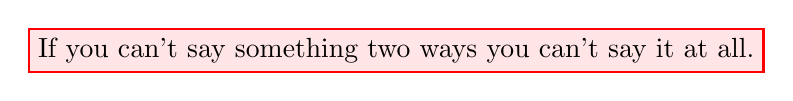
\begin{tikzpicture}
        \node[draw=red, fill=red!10, thick]
            {If you can't say something two ways you can't say it at all.};
    \end{tikzpicture}
\end{center}

This credo may seem odd to linguists, who usually take a strongly realist stance according to which the grammar formalism fully specifies the grammar, even down to notation.
For example, privative (= single-valued) and binary features are regarded as vastly different objects that make very different claims about phonology.
Yet we will see at a later point that they are but two definitions of the same computational object.
That does not rule out that one of the two is a more useful way of thinking about phonology, but that is a matter of epistemology rather than ontology.

\begin{definition}[Bigrams]
    Given a string $w$ over alphabet $\Sigma$, its \emph{augmented} counterpart $\augmented{w} \is \LeftEdge \stringcat w \stringcat \RightEdge$ is obtained by adding the left and right edge markers $\LeftEdge$ and $\RightEdge$ to $w$, where $\LeftEdge$ and $\RightEdge$ are distinguished symbols not contained in $\Sigma$.
    Furthermore, 
    \(
    \Bigrams(w) \is
        \setof{
            \ngram{ab} \mid \exists u,v \in \Sigma^* \text{ s.t.\ }
                u \stringcat \ngram{ab} \stringcat v = \augmented{w}
        }
    \)
    denotes the set of \emph{bigrams} over $\augmented{w}$, i.e.\ the smallest set that contains all substrings of $\augmented{w}$ that consist of exactly $2$ symbols.
\end{definition}

\begin{definition}[Bigram Grammar]
    A \emph{bigram grammar} $G$ over alphabet $\Sigma$ is a finite set of bigrams over $\Sigma \cup \setof{\LeftEdge, \RightEdge}$.
    If $G$ is a \emph{positive bigram grammar} (denoted $\posG{G}$), then it generates the language
    \(
        L(G) \is \setof{
            w \mid \Bigrams(w) \subseteq G
        }
    \).
    If $G$ is a \emph{negative bigram grammar} (denoted $\negG{G}$), then it generates the language
    \(
        L(G) \is \setof{
            w \mid \Bigrams(w) \cap G = \emptyset
        }
    \).
\end{definition}

With all these definitions under our belt, we can finally move on to producing a new insight: positive and negative bigram grammars are equally powerful.
That is to say, if some language is generated by a positive bigram grammar, then it can also be generated by some negative bigram grammar, and the other way round.

\begin{theorem}
    The class of languages that are generated by positive bigram grammars is exactly the class of languages that are generated by negative bigram grammars.
    \label{thm:SL_PosNegEquivalence}
\end{theorem}
%
In order to show that this theorem is indeed correct, we establish two simpler propositions --- called lemmata --- which jointly imply the theorem.

\begin{lemma}
    For every positive bigram grammar there is a negative bigram grammar that generates the same language.
    \label{lem:SL_Pos2Neg}
\end{lemma}
%
\begin{proof}
    Let $\posG{G}$ be a positive bigram grammar. 
    We show that $\negG{\complementof{G}}$ defines the same language as $\posG{G}$, where $\complementof{G}$ consists of all bigrams over $\Sigma \cup \setof{\LeftEdge, \RightEdge}$ that are not contained by $G$.

    Pick some arbitrary string $w \in L(\posG{G})$. 
    By definition, every bigram of $w$ is a member of $G$, which immediately implies that no element of $\Bigrams(w)$ is contained in $\complementof{G}$.
    But if none of the bigrams of $w$ belong to $\complementof{G}$, then $\Bigrams(w) \cap \complementof{G} = \emptyset$, wherefore $w \in L(\negG{\complementof{G}})$.
    Since $w$ was arbitrary, this result holds for every string generated by $\posG{G}$, establishing $L(\posG{G}) \subseteq L(\negG{\complementof{G}})$.

    The same argument can be applied in the other direction to show $L(\posG{G}) \supseteq L(\negG{\complementof{G}})$, wherefore $L(\posG{G}) = L(\negG{\complementof{G}})$.
\end{proof}
%
This is a so-called \emph{constructive} proof: we do not just show that an equivalent negative bigram grammar exists, we also explain how this grammar can be constructed from the positive bigram grammar.
Constructive proofs are the most useful kind of proof because they provide procedures and strategies that can be implemented and run automatically.

In the case at hand, all we have to do in order to construct an equivalent negative bigram grammar is to take the set-theoretic complement of the positive bigram grammar.
After all, the set of all bigrams over $\Sigma$ is given by $\Sigma \times \Sigma$, and the positive bigram grammar $\posG(G)$ is some subset thereof (\emph{modulo} edge markers, which are treated as part of $\Sigma$ here to avoid notational clutter).
Bigrams that belong to $G$ may occur in a string, bigrams that do not must not.
So the bigrams not belonging to $G$ are the illicit bigrams, which means those are exactly the bigrams the equivalent negative bigram grammar must contain.
In one sentence: taking the complement of $G$ is like taking its negation, and the switch from a positive grammar to a negative one undoes this negation.

So now we know that the negative bigram grammars are at least as powerful as the positive bigram grammars since the latter can be translated into the former.
It only remains for us to show that the same holds in the other direction.

\begin{lemma}
    For every negative bigram grammar there is a positive bigram grammar that generates the same language.
\end{lemma}
%
\begin{proof}
    Left as an exercise to the reader.
\end{proof}

\subsection{The How and Why of Proofs}

Proofs are a difficult art at every level of expertise.
For the beginner, the biggest challenge is often to sort out their train of thought and present it in a clear manner: where do I start, and how do I proceed from there step by step to reach the conclusion?

There are no clear-cut rules here, but it is often helpful to break up the problem into smaller ones, as we did with Thm.~\ref{thm:SL_PosNegEquivalence}.
If two sets $A$ and $B$ need to be shown to be equivalent, one can first prove $A \subseteq B$ and then $B \subseteq A$.
And a statement of the form ``$\phi$ iff $\psi$'' can be broken up into ``$\phi$ entails $\psi$'' and ``$\psi$ entails $\phi$''.
We will encounter several basic proof techniques throughout the course (proof by induction, indirect proofs), but don't worry too much about specific techniques for now.
Instead, make sure to work through the proofs we discuss multiple times until you understand how they work.
Always try to answer the following questions for yourself:

\begin{itemize}
    \item Why is the initial assumption valid?
    \item How does each conclusion follow from the previous one?
    \item Why does the final conclusion show that the theorem\slash lemma is correct?
\end{itemize}

You may wonder why we need proofs in the first place.
Linguists don't work with proofs yet they have discovered a lot of interesting things about language.
Programmers don't have much use for proofs either.
There's several answers, the simplest one being that some questions can only be addressed conclusively via proofs.
Consider the following alternative to the proof of Lem.~\ref{lem:SL_Pos2Neg}: we could have implemented the translation procedure from positive to negative grammars and then tested it on a large sample of positive bigram grammars (at least several thousand).
Eventually the program would have told us that the negative grammars generate the same string languages as their positive counterparts.
So if the conversion works correctly on every single one of thousands of positive bigram grammars, isn't that enough to posit that positive and negative bigram grammars are interchangeable?

The answer is No.
First of all, checking that two grammars generate the same language is hardly trivial if both languages are infinite (we can't just compare all their respective members).
More importantly, though, the thousands of test grammars may accidentally share a special property that is essential for the correctness of the conversion.
This is a real risk if all those test grammars were automatically generated by a script because true randomness is very hard to achieve with computers, if not impossible.
While experiments and simulations have their place --- they are a valid last resort where proofs are hard to come by --- a proof is always the preferred solution where possible.

Proofs are preferred not only because they are safe from the pitfalls of simulations, but also because they provide genuine insight.
In fact, proofs are often more important and enlightening than the theorems they establish.
Testing the correctness of the bigram conversion via automated experiments could at best show us whether the procedure is correct (if there's only finitely many cases to test), but it does not tell us \textbf{why}.
A proof is an explicit record of how certain properties entail others.
In the case at hand, it is the close connection between set-theoretic complementation and the switch from positive to negative grammars that does all the work.
Notice all the properties of bigram grammars that the proof does not depend on: that bigrams are strings, that bigrams consist of exactly two symbols, and that bigram grammars are finite. 
Yet these properties necessarily hold during any test procedure, so we would not be able to tell which one of them is a prerequisite for the correctness of the conversion.
Thanks to the proof, we know which properties matter, which in turn might come in handy in the study of other formalisms.

In a few lines, a proof can establish unassailable truths, show us why they hold, but also save us hours of work compared to running simulations.
So even though you may initially find them hard and time consuming, proofs are actually the tool of choice for the lazy scientist.


\section{Linguistic Evaluation}
The bigram grammar model improves on the list phonology model in various respects.
Variation across languages is now much more restricted because phonology is just a collection of highly local constraints (negative bigram grammars) or permissions (positive bigram grammars).
Bigram grammars also account for linguistic creativity, i.e.\ that speakers can form new words according to the rules of their own language, and that they recognize whether nonce words are well-formed.
As a consequence, they do not predict that the lexicon is finite, either.
Whether the lexicon is finite or infinite is immaterial for bigram grammars since they determine well-formedness in a compositional manner.
As long as each word is finite, its grammaticality can easily be determined via a bigram scanner.

Bigram grammars do still exhibit isolationism and egalitarianism.
Since a grammar is a list of bigrams, all these bigrams should have the same status and there should be no distictions between easy and difficult processes.
And processes still cannot apply across words: for \emph{phone bill}, the phonological representation is presumably something like \LeftEdge\textipa{foUn}\RightEdge\LeftEdge\textipa{bIl}\RightEdge.
Since \textipa{n} and \textipa{b} are not adjacent, a negative bigram grammar with \ngram{nb} does not have the desired result.
This could be fixed with a bigger search domain, though, which also seems to be necessary for slightly less local processes like intervocalic voicing, where we want to block a voiceless sound only if it occurs between two vowels.

Overall bigram grammars are doing very well on a conceptual level and are easy to implement, but they are not expressive enough for English.
Next time we will see how we can keep all their attractive properties while increasing their power to a more adequate level.

%hw: does this model have smaller memory usage? By how much?

\chapter{Learning Local Dependencies}
\label{cha:LearnSL}

Strictly local grammars provide a model for local phonological processes that is sufficiently powerful (all local processes can be correctly described), cognitively plausible (low memory load, efficient runtime behavior), and captures some essential properties of natural language phonology (linguistic creativity, generalization from short strings to longer ones, some processes are more complex than others, constraints can apply conjunctively but not disjunctively).

Even in the best case, though, this is insufficient to attain full \emph{explanatory adequacy} in the terminology of \citet{Chomsky65}.
Recall the three levels of adequacy:
%
\begin{enumerate}
    \item \textbf{Observational Adequacy}\\
        The theory correctly accounts for all the observed data.
    \item \textbf{Descriptive Adequacy}\\
        The theory describes a native speaker's knowledge of their language.
        Hence it gives a full specification of their grammar and thus makes the right predictions even for unobserved data.
    \item \textbf{Explanatory Adequacy}\\
        The theory explains how a native speaker acquires their knowledge from the primary linguistic data.
\end{enumerate}
%
Strictly local grammars are certainly observationally adequate since they can handle every phonological process as long as its application domain is bounded in size.
Descriptive adequacy requires the formal model to mirror the speaker's internal grammar; a standard which is rather hard to evaluate.
At the very least strictly local grammars can generalize beyond finite data, make typological claims, and offer a rigorous definition for what grammars look like (they are finite sets of $n$-grams).
So they certainly go beyond observational adequacy and might even be descriptively adequate --- provided that phonology involves no mappings from underlying forms to surface forms, which is something these grammars do not handle.

Explanatory adequacy is all about the acquisition of the grammar.
\Note{%
    Linguists commonly use the term explanatory adequacy in a more general sense nowadays to describe any kind of account that explains a given phenomenon rather than just stipulating a grammar with a bunch of properties that correctly account for the data.
Chapter 1 of \citet{Chomsky65}, on the other hand, clearly ties it to matters of learnability.
}
Given a (possibly infinite) collection of grammars to choose from, how does a speaker arrive at a descriptively adequate grammar from a finite sample of input data?
This is an issue we haven't addressed at all yet. 
As we will see today, strictly local grammars can be learned rather easily given that a crucial piece of information is already specified via our genetic endowment (i.e.\ Universal Grammar in generative terminology).
So strictly local grammars do offer a nativist account of how local phonological processes can be acquired.

\section{Machine Learning versus Learnability}

The question of how grammars can be learned is also of great in computational linguistics and NLP\@.
On a purely practical level, it isn't feasible to hand-write grammars for all the languages in the world, not even if we only focus on their phonology.
And even if that were possible, hard-coded grammars cannot adapt to local dialects or ongoing changes in the speech community.
So it is preferable to have an algorithm that constructs and modifies grammars based on the input it gets.
The development, evaluation, and efficient deployment of such algorithms is the purview of \emph{machine learning}.

Unsuprisingly, learning algorithms that work well in real-world applications are very complex beasts that can be hard to understand and analyze.
So it is often more insightful to study a more abstract problem: given a possibly infinite space of languages, can we identify properties of this space that guarantee the existence of a learning algorithm provided certain types of input?
This question is studied in \emph{learnability}.

Just like the difference between computational linguistics and NLP, the difference between learnability and machine learning is often subtle.
The most important distinction, however, is that learnability is not about learning but rather about studying the structural properties of language classes and how one they facilitate generalization.

In a certain sense, learnability is linguistics as the level of languages rather than the objects these languages describe.
In linguistics, we identify structural generalizations for sentences and words, encoded via a grammar, that can be invoked to determine well-formedness and make typological predictions.
In learnability, we also identify structural generalizations, but we do not look at the objects within a language but rather at all languages within a given class.
More formally, linguistics looks at sets of objects, and learnability looks at sets of such sets.
This point of view highlights that learnability is not directly concerned with learning as such, although its result have important ramifications for learning (just like computational linguistics is not about processing language with computers but its results can be applied this way).

Machine learning, on the other hand, is about solving any kind of problem that involves a learning component.
This naturally makes it a much messier affair.
If you want to teach a computer to filter spam mails, that is a learning problem, but it is not obvious how one could formalize this learning problem or what it even means for the learner to work correctly --- although it is very easy to tell for the user when their spam filter screwed up.
At any rate the problem certainly isn't approached in terms of, say, a space of spam languages and how its properties can be exploited for learning.
That's not so say that such considerations never factor into the initial design of the learning algorithm, but they are not the central object of study.

There are also huge methodological differences between learnability and machine learning.
Learnability is all about mathematical theorems and proofs, whereas experiments and simulations are much more common in machine learning.
Just like with computational linguistics versus NLP, that is often a matter of necessity: the learning algorithms used in machine learning are so complex, and the problems so difficult to define in formal terms, that proofs simply aren't feasible.
And of course machine learning has a stronger focus on solving real-life problems, so pretty much anything goes as long as it gets the job done, even if nobody can tell why it gets the job done.

So which one of the two perspectives, learnability or machine learning, is more insightful for linguistics?
It depends on what kind of linguistics we have in mind.
Linguistic performance is a tricky problem with lots of noise, few clear-cut generalizations, and no clear success state for the learner, so a problem like, say, speakers' use of slang words and how it is contingent on the social setting is probably better off with machine learning.
Linguistic competence, on the other hand, is sufficiently abstracted that we can have rigorous mathematical definitions of the object of study and what it means to successfully solve a given learning problem.
And since mathematical proofs offer the highest standard of truth that we should strive for whenever possible, learnability is the better perspective for our purposes.

\section{A Closer Look at Learnability}

\subsection{General Remarks on Learning}

The definition of explanatory adequacy given at the beginning require the theory to explain how a native speaker acquires their grammatical knowledge.
But what exactly does that mean?
For the sake of simplicity, let's assume that ``explain'' here just means that we have a learning algorithm, or simply \emph{learner}.
Chomsky might have had a stronger condition in mind, e.g.\ that the learner must somehow be defined via the grammar formalism, but with highly abstract issues like this it is always more instructive to consider the simplest case first before piling on additional complicating factors.
Assuming then that any learner will do, what exactly is it the learner has to accomplish?
What does it mean to acquire grammatical knowledge, how can we translate that into a mathematical statement?

There are of course many perfectly valid answers to this, so we will have to choose between these alternatives according to what exactly it is we are interested in.
First of all, there are two ways of thinking about acquiring grammatical knowledge: learning a language, and learning the grammar for that language.
In the first case, a learner of phonology just has to arrive at a state where one can tell for every word whether it is well-formed.
In the second case, the learner must also use the right grammar.
This is usually how linguists think about acquisition, but it is a rather curious notion because many grammars generate exactly the same language.

For example, if $G$ is a strictly $2$-local grammar, and $G' \is G \cup \setof{\RightEdge \LeftEdge}$, then the two generate exactly the same language because $\RightEdge\LeftEdge$ is a useless bigram, it never occurs in any string.
So a learner that acquires $G'$ instead of $G$ is still learning the correct language, only the grammar is slightly larger than it needs to be.
Similarly, if strictly local grammars are actually formalized as lists rather than sets, then two grammars can be distinct despite containing exactly the same $n$-grams just because the order of $n$-grams differs.
So for every grammar $G$ there are $(\cardof{G}-1)!$ many alternative grammars that generate exactly the same language.
As a result there is no way to distinguish among these grammars based on well-formedness judgments.

The tacit assumption among linguists is that in such cases smaller grammars are to be preferred, and that differences in grammar can be detected with more sophisticated methods, e.g.\ psycholinguistic experiments.
But the first one is a stipulation at best and a category mistake at one: while it is true that as scientists we should strive to find the simplest solutions and thus the smallest grammar, it is far from obvious that this scientific principle should be a condition on the learner.
There are many cases where constructing a grammar for a formal language is possible yet one cannot determine whether there is a smaller grammar.
If grammar size is an important factor in distinguishing adequate from inadequate learners, explanatory adequacy is unattainable under such circumstances.
So if human language happens to be such a case, explanatory adequacy could never be achieved, which seems rather odd.
The natural conclusion, then, is that grammar size is not an essential criterion.

The second assumption is that grammars can be distinguished even if they generate exactly the same language.
Given a suitable linking theory between competence and performance, it is indeed conceivable that two grammars may make different predictions, e.g.\ in parsing, word recognition or possibly even the brain patterns on can observe.
But to date there is no consensus on what such a linking theory has to look like, and more importantly, we do not know that speakers all have the same grammar in this sense.
For example, whether a somebody is right-handed or left-handed has a profound difference on brain function, so we cannot rule out that right-handed people's grammars are different from that of left-handed people.
Similarly, a psycholinguistic experiment such as a reading tasks does not measure the grammar in isolation but rather the compound output of working memory load, attention span, and so on.
Unless there is a way to control for all these variables to a level of degree where one can detect even subtle differences in grammar, there is no evidence that speaker's learn the same grammar.
In fact, behavioral data suggests the opposite: even when speakers agree on all relevant data judgments for a given phenomenon, they can still have different preferences for certain structures, or they may be more likely to use one than the other.
Overall, then, there is no strong reason why ``acquiring grammatical knowledge'' must mean finding the right grammar rather than the right language.

Another important factor missing from the definition of explanatory adequacy are the parameters of learning, i.e.\ what kind of evidence the learner can draw from and how quickly learning must proceed.
If our main interest is modelling human learning, then those issues are first and foremost an empirical matter, and whatever is available to an infant learner should also be available to our formal learner.
The problem, though, is that it often unclear what evidence infants can draw from.
We know for sure that they get positive evidence by virtue of constantly being exposed to natural language input.
But they might also have access to negative evidence, for if you never hear a specific form or construction, that makes for strong probabilistic evidence that it is ill-formed.
Setting aside the question of what counts as input, we also do not know how much information is extracted from that input.
The actual surface forms --- sequences of sounds for phonology, sequences of words for syntax --- are definitely accessible, whereas it is much less clear how much syntactic structure can be inferred from prosody and semantics.
The only thing we know for sure, then, is that language acquisition involves at least collections of surface forms.
The best starting point, then, is to see what can or cannot be learned with such a restricted amount of information.


\subsection{The Gold Paradigm}

The learnability literature is full of different learning paradigms that make varying assumptions about the input available to the learner and the criteria that determine learning success.
One of the oldest and most influential is the \emph{Gold paradigm}, also known as \emph{learning in the limit} or \emph{learning in the limit from positive text}.
The Gold paradigm makes very minimal assumptions about the input while enforcing a very strict notion of learning success.
The learner is presented with strings from the target language, one after another.
After each string presentation the learner formulates a theory (represented by a grammar) as to what language that string was drawn from.
The learner is successful iff it guesses the right language after a finite number of steps and, crucially, does not change its guess at a later point.

Let us make these ideas more precise so that we know what exactly we are talking about before moving on.
%
\begin{definition}[Text]
    Given a language $L$, a \emph{(positive) text} over $L$ is a total mapping $T$ from the natural numbers onto $L \cup \setof{\Noise}$ (that is to say, it is an infinite string in which ever member of $L$ occurs at least once and random noise is represented by \Noise).
    We denote by $T(i)$ the $i+1$-th element in the text, whereas $T[i]$ represents the length $i$ prefix of $T$, i.e.\ $\tuple{T(0), T(1), \ldots, T(i-1)}$.
    For every sequence $s$, $\contentof(s)$ is the set of elements of $L$ that occur in $s$.
\end{definition}
%
\begin{definition}[Gold learning]
    A \emph{learner} is a (possibly partial) function $\Learner$ from sequences of expressions and \Noise\ to languages.
    The learner \emph{converges} on text $T$ iff there is some $i$ such that $\Learner(T[i]) = \Learner(T[j])$ for all $j \geq i$.
    The learner \emph{identifies} language $L$ iff it holds for every text $T$ over $L$ that \Learner\ converges on $T$ and guesses the correct language (that is to say $L(\Learner(T)) = \contentof(T)$).
    Similarly, \Learner\ identifies a class $\mathcal{L}$ of languages iff it identifies every language in that class.
    A class of languages is \emph{identifiable} or \emph{learnable (in the limit)} iff there is a learner that identifies it.
\end{definition}
%
\begin{examplebox}[Every Language is Learnable]
    Here is a quick example that shows all the terminology and concepts of Gold learning in action.
    It also illuminates a common source of confusion: learnability is a property of language classes, not individual languages.
    When considered in isolation, every language is learnable.

    Let $L$ be some language.
    We show that $\setof{L}$ is learnable in the limit by exhibiting a learner that identifies $\setof{L}$.
    This learner is the constant function \Learner\ such that for every expression $i$ $\Learner(i) \is L$.

    Since \Learner\ is a constant function it makes the same guess for every prefix of any text $T$ over $L$, so we have $\Learner(T[i]) = L$ for every $i \geq 0$.
    This immediately implies that the learner converges on $T$, and since $T$ is drawn from $L$ we also have that $L(\Learner(T)) = \contentof(T)$.
    This will be the case for every text $T$ over $L$, so \Learner\ identifies $L$, which means that it also identifies the class $\setof{L}$.
\end{examplebox}
%
The order of steps in the example is representative of learnability proofs in general.
%
\begin{enumerate}
    \item Give a learner.
    \item Show that the learner converges, that is to say, it does not alter its guess after a certain point.
    \item Show that after it converges, the learner correctly guesses the target language.
        In other words, it identifies the language.
    \item Show that the learner can do this for all languages in the class and all texts over them. 
\end{enumerate}

At this point you might already have a hunch that the Gold paradigm is not a fully realistic representation of language acquisition.
You would be right, many factors are omitted or simplified.
There are no constraints on how quickly a learner has to converge, so a learner that takes 300 years to find the target language is perfectly acceptable.
The learner also has perfect recall since its guess at position $i$ in the text is not just determined by the element at this position, which we denote $T(i)$, but by all the elements up to this position, which is represented by the minimally different $T[i]$.
These two factors simply the learning problem a lot.

At the same time, some factors probably make the Gold paradigm harder than the real life task.
In particular, the learner has to succeed on every text, no matter how defunct and degenerate that text is.
It is highly unlikely that a child could learn from input that consists predominantly of sentences from Wall Street Journal op-ed pieces --- child-directed input starts out easy with simple short sentences and increases gradually in complexity.
The Gold paradigm requires the learner to succeed even under highly adversarial circumstances.
And the restriction to strings that are completely stripped off prosody and semantics also heightens the difficulty of the task.

It is important to keep in mind though that these aren't so much issues of empirical inadequacy as they are consequences of mathematical abstraction.
By keeping the paradigm as simple as possible, we can get insight into why certain classes of languages are learnable and others are not, and these insights can be adapted to more adequate paradigms in subsequent work.
The process isn't all that different from what we are currently doing in our analysis of phonology: set out the bare essentials that need to be accomplished, see how one might go about this with the least amount of assumptions, and where necessary revise the model in a conservative fashion so that one can easily tell which properties are being preserved, and why.


\subsection{Most Classes of Languages are not Learnable}

One of the key insights of the Gold paradigm is that a surprisingly large number of language classes is not learnable.
More precisely, ever proper superset of the class of finite languages is not identifiable in the limit.
This is even more surprising because the class of finite languages is learnable.
%
\begin{theorem}
    The class $\FIN$ of finite languages is identifiable in the limit.
\end{theorem}
%
The key idea is that every finite language can be learned within a finite number of steps by simply memorizing all the forms encountered so far.
Remember that this was our original idea for the list phonology model, so this theorem tells us that list phonology is a learnable model of phonology.
%
\begin{proof}
    Let $\Learner$ be a function that, for every text $T$ and index $i$, maps $T[i]$ to $\contentof(T[i])$.
    For every finite language $L$ and text $T$ over $L$, there must be a smallest $i$ such that $\contentof(T[i]) = L$.
    Thus $\Learner(T[i]) = \Learner(T[j])$ for all $j \geq i$, wherefore the learner converges on $T$.
    But we also have $\Learner(T[i]) = \contentof(T[i]) = L$, and since $T$ was arbitrary $\Learner$ identifies $L$.
    But $L$, too, was arbitrary, showing that $\Learner$ identifies $\FIN$.
\end{proof}


The learner used in the proof is rather boring because it only memorizes forms without any kind of generalization --- one of the biggest qualms we had with list phonology model.
But generalization is risky as it involves formulating a hypothesis that goes beyond the mere data.
Depending on how the space of languages is structured, it may be more or less safe to generalize in certain ways.
In the worst case, safe generalization is impossible, and that is exactly the problem with any language class that properly includes all finite languages.
%
\begin{theorem}
    Every class of languages that properly subsumes $\FIN$ is not identifiable in the limit.
\end{theorem}
%
Note that every class of this type must include at least one infinite language.
So a learner that tries to learn this class must guess this infinite language after having seen only a finite amount of data --- that's the convergence criterion.
But there is no guarantee that this finite amount of data isn't actually sampled from a finite language that is included in the infinite one, in which case the learner would have accidentally overgeneralized.
Since there is no negative evidence in the Gold paradigm, the learner has no opportunity to revise its decision and makes the wrong guess.
%
\begin{proof}
    We show that $\mathcal{L} \is \FIN \cup \setof{L}$ is not identifiable, where $L$ is some infinite language.
    This immediately implies that no proper superset of $\FIN$ can be identified in the limit.

    Suppose that $\Learner$ identifies $\mathcal{L}$.
    Then $\Learner$ must identify every member of $\mathcal{L}$, including $L$.
    By definition, then, it must hold for every text $T$ over $L$ that there is some $i$ where $\Learner$ converges on $T$.
    Clearly $\contentof(T[i])$ is a finite language $F$.
    Let $T_F$ be a text over $F$ such that $T_F[i] = T[i]$.
    Then $\Learner$ must also converge on $T_F$ at index $i$, but since $\Learner$ identifies $L$ over $T$ it must be the case that $\Learner(T_F)$ is $L$ rather than $F$.
    So $\Learner$ does not identify $F$ over $T_F$, wherefore it does not identify $F$ or $\mathcal{L}$ either.
\end{proof}

The two theorems home in on the central problem of learning a given space of languages in the Gold paradigm: on the one hand the learner has to generalize from a finite amount of input to an infinite language, but on the other hand this generalization step needs to be conservative enough that the learner can avoid from overgeneralization.
Other learning paradigms usually give the learner some means of recovering from overgeneralization to some degree --- e.g.\ via probabilistic reasoning, negative evidence, or an all-knowing oracle that can be asked specific questions --- but the tension between finite data and infinite target languages remains.
This tension can be resolved correctly only if the space is structured in a specific way and the learner is aware of that structure.

There are some clear parallels to Universal Grammar (UG) in linguistics.
However, UG does not really talk about the structure of the language space but rather puts restrictions on what the elements of each language in that space look like.
By itself that is not enough to guarantee learnability.
Nonetheless UG considerations and learnability can be linked in intriguing ways, as we will see next in our look at the (non-)learnability of strictly local languages.

\section{Learning Strictly Local Languages}

\subsection{\texorpdfstring{$\SL_k$ is Learnable}{SLk is Learnable}}
%
Remember that the class of strictly local languages properly subsumes the class of all finite languages, so this immediately tells us that the full class is not Gold-learnable.
%
\begin{corollary}
    $\SL$ is not identifiable in the limit.
\end{corollary}

But the full class of strictly local languages isn't all that interesting for our purposes anyways.
By definition there is an upper bound $k$ on the domain of local phonological processes, otherwise they would be non-local processes.
It seems reasonable that the value of $k$ is part of UG so that human learners only entertain hypothesis that fall within the realm of strictly $k$-local languages (or maybe there is some language external factor that limits the class of hypothesis to $\SL_k$; at any rate there is some learning prior in place).
And in contrast to $\SL$, $\SL_k$ is learnable for every choice of $k$.
%
\begin{theorem}
    $\SL_k$ is identifiable in the limit for every $k \geq 0$.
\end{theorem}
%
By now you probably know already what the learner has to do: memory all $k$-grams of all strings seen so far.
%
\begin{proof}
    Let $\Learner_k$ be such that for every text $T$ of strictly $k$-local language $L$, $\Learner_k(T[i]) = L(G)$, where $G \is \bigcup_{w \in \contentof(T[i])} \Bigrams[k](w)$ is a positive strictly $k$-local grammar.
    Since there are only finitely many distinct $k$-grams, $\Learner_k$ is guaranteed to converge at some index $i$.
    At this point, $G$ contains all $k$-grams that occur in some string in $T$, and only those, so $L(G) = L$.
    Since $L$ and $T$ were arbitrary, $\Learner_k$ identifies $\SL_k$.
\end{proof}

While the result is stated in terms of learning, we can also view it as a description of the language space that $\Learner_k$ induces.
That is to say, given some finite input sample, $\Learner_k$ will generalize to a (possibly infinite) language, namely the smallest strictly $k$-local language that includes the input.
So if all phonological dependencies are strictly $k$-local, that might not necessarily be due to a restriction of the grammar.
Maybe phonological computations could work just as well with much larger values, or even the whole class of strictly local languages.
But the learner $\Learner_k$ only infers $\SL_k$-grammars.
No matter what input it is presented with, it will always generalize to a specific type of grammar.
This allows us to factor language as an empirical object into at least two distinct components: the class of languages that can be generated by the grammar formalism, and the class of languages that are identified by the learner.
Natural languages are the special type of language that belongs to both.
So you see, learnablity is not just tied to language acquisition, it can also be invoked to explain typological facts.


\subsection{Generalizing the Learner}
The proof that $\SL_k$ is identifiable in the limit is deceptively simple.
In just five lines it establishes the learnability result, but it does not quite home in on why this works, what aspects of strictly local languages are essential for the proof, and what exactly the explored space looks like.
These are important points; if we want to revise our formalism at some later point without losing the learnability property, we need to know what we can safely change.

Let's first think about the overall shape of $\SL_k$.
One useful trick is to identify each language with a grammar that generates it and think about that space of grammars instead.
After all, one is just a different representation of the other.
Suppose we are interested in the strictly $1$-local languages over $a$ and $b$.
There are 4 different 1-grams over this alphabet: $\LeftEdge$, $\RightEdge$, $a$, and $b$. 
Since every strictly $1$-local grammar is a set of these $1$-grams, the class of $\SL_1$ grammars over $a$ and $b$ is the powerset of the set of these $4$ bigrams.
This means that there are $2^4 = 16$ different $\SL_1$-grammars, and these grammars are partially ordered by the subset relation.
We can actually represent this space graphically as in Fig.~\ref{fig:LearnSL_SL1-Lattice}.
%
\begin{figure}[htpb]
    \centering
    \begin{tikzpicture}
    % Lattice of SL1-grammars over alphabet {a,b} with edge markers

    % atoms
    \node (a) at (0,0) {$\setof{a}$};
    \node (b) [right=of a] {$\setof{b}$};
    \node (L) [left=of a] {$\setof{\LeftEdge}$};
    \node (R) [right=of b] {$\setof{\RightEdge}$};

    % level 2
    \node(La) [above left=of L] {$\setof{\LeftEdge, a}$};
    \node(Lb) [above=of L] {$\setof{\LeftEdge, b}$};
    \node(LR) [above=of a] {$\setof{\LeftEdge, \RightEdge}$};
    \node(ab) [above=of b] {$\setof{a,b}$};
    \node(aR) [above=of R] {$\setof{a, \RightEdge}$};
    \node(bR) [above right=of R] {$\setof{b, \RightEdge}$};

    % level 3
    \node(Lab) [above=of Lb] {$\setof{\LeftEdge, a, b}$};
    \node(LaR) [above=of LR] {$\setof{\LeftEdge, a, \RightEdge}$};
    \node(LbR) [above=of ab] {$\setof{\LeftEdge, b, \RightEdge}$};
    \node(abR) [above=of aR] {$\setof{a, b, \RightEdge}$};

    % top and bottom
    \node[xshift=2.5em] (1) [above=of LaR] {$\setof{\LeftEdge, a, b, \RightEdge}$};
    \node[xshift=2.5em] (0) [below=of a] {$\setof{}$};

    % branches    
    % bottom level
    \foreach \Source in {a,b,L,R}
        \draw (\Source) to (0);

    % top level
    \foreach \Target in {Lab,LaR,LbR,abR}
        \draw (1) to (\Target);

    % level 2 via atoms
    \foreach \One/\Two in {L/a,L/b,L/R,a/b,a/R,b/R}
        {
        \draw (\One) to (\One\Two);
        \draw (\Two) to (\One\Two);
        }

    % level 3 (not as nicely abstracted as level 2)
    \foreach \Target in {La,ab,Lb}
        \draw (Lab) to (\Target);

    \foreach \Target in {La,aR,LR}
        \draw (LaR) to (\Target);

    \foreach \Target in {Lb,bR,LR}
        \draw (LbR) to (\Target);

    \foreach \Target in {ab,bR,aR}
        \draw (abR) to (\Target);
\end{tikzpicture}

    \caption{Lattice representation of the space of $\SL_1$-grammars over $a$ and $b$}
    \label{fig:LearnSL_SL1-Lattice}
\end{figure}

As you can see this space has a lot of structure.
First of all, there are unique bottom and top elements, which are $\setof{}$ and $\setof{\LeftEdge, a, b, \RightEdge}$ in this case.
It also holds that any two nodes have a unique greatest lower bound (\emph{infimum}) and a unique least upper bound (\emph{supremum}).
For example, $\setof{\LeftEdge,a}$ and $\setof{\LeftEdge,b}$ have the greatest lower bound $\setof{\LeftEdge}$ and the least upper bound $\setof{\LeftEdge,a,b,}$.
A partially ordered set where all nodes $x$ and $y$ have both an infimum and a supremum is called a \emph{lattice}, and if it also has unique bottom and top elements it is a \emph{bounded lattice}.

It is fairly easy to see that the class of $\SL_k$ grammars always forms a bounded lattice, the size of which depends on $k$ the number of symbols in the alphabet.
For example, there are $9$ distinct bigrams over $a,b$ (strictly speaking there are more, like $\RightEdge a$, but those can never occur in a string), so the corresponding lattice has $2^9 = 512$ distinct nodes, which is way too much to draw.
Still, they are all lattices.

The strategy used by $\Learner_k$ can be viewed as a particular way of moving through such a lattice.
The learner starts at the bottom of the lattice and the moves upwards whenever the current input cannot be accounted for by the grammar represented by the current node in the lattice.
In the specific case of $\SL_k$ learning, this means that the input string contains a $k$-gram that is not part of the current grammar.
Crucially, though, the learner can determine the shortest upward move that will take it to a grammar that can deal with all the input so far.
Suppose that $\Learner_1$ is currently at the node $\setof{\LeftEdge, a, \RightEdge}$ and is now presented with the input $b$.
That string is not generated by the grammar $\setof{\LeftEdge, a, \RightEdge}$, as its set of $1$-grams is $\setof{\LeftEdge, b, \RightEdge}$.
The learner infers from this that the grammar is $\setof{\LeftEdge, a, b, \RightEdge}$, but notice what is happening in the lattice:
the learner isn't just moving upwards, it's moving to the supremum of the nodes that correspond to these two grammars!

By moving to the supremum rather than just any random higher node, the learner generalizes in the most careful and conservative way possible that is consistent with the data, which avoids overgeneralizing.
If the supremum isn't the right grammar, then there will be more evidence further down the line and we can move to the next higher supremum, and so on.
If, on the other hand, the learner simply moved to some arbitrary higher node, there would be no evidence that it has the wrong grammar and no way for it to correct its mistake.

The lattice-based learning perspective is so appealing because it is both intuitive and general.
It doesn't really matter that the nodes in the lattice correspond to strictly local grammars, what matters is that the learner has a way to explore this space in a principled fashion without overgeneralizing.
This can be done as long as the learner can derive a second node from the input such that the supremum of that second node and the learner's current position corresponds to the most conservative revision of the learner's current hypothesis that can account for all the input so far.
So if a given class of languages can be shown to have a lattice structure, and if we can define a method for picking the right suprema, then we have a learner for that class of languages.

This is also highly appealing from a psycholinguistic perspective since one would assume that learning strategies do not differ significantly for, say, local and non-local phonological processes.
Once we move from local to non-local processes, we will see that this is indeed the case: both processes involve exactly the same lattice-based learning algorithms,  with the only difference being what each lattice represents.
%hw: construct corresponding lattice for SL1 languages; what is the mapping depending positive or negative grammar?

\chapter{Beyond Well-Formedness}
\label{cha:PSL}

\begin{itemize}
    \item probabilistic version: switch to different monoid (0,1,min; 0,1,*; [0,1],*)
    \item inferring probabilities
    \item smoothing techniques
\end{itemize}

\begin{align*}
    f(aba) & =
            f(\LeftEdge a)
            \times
            f(ab)
            \times
            f(ba)
            \times
            f(a\RightEdge)
            \\
            & =
            1
            \times
            1
            \times
            1
            \times
            0
            \\
            & =
            0
\end{align*}

\begin{center}
    \begin{minipage}{.35\linewidth}
        \begin{align*}
            f(aba)
            &= 1 \times (1 \times (1 \times 0)) \\
            &= 1 \times (1 \times 0) \\
            &= 1 \times 0\\
            &= 0
        \end{align*}
    \end{minipage}
    %
    \begin{minipage}{.2\linewidth}
        \begin{align*}
            &= 1 \mathrel{\text{min}} (1 \mathrel{\text{min}} (1 \mathrel{\text{min}} 0)) \\
            &= 1 \mathrel{\text{min}} (1 \mathrel{\text{min}} 0) \\
            &= 1 \mathrel{\text{min}} 0\\
            &= 0
        \end{align*}
    \end{minipage}
    %
    \begin{minipage}{.25\linewidth}
        \begin{align*}
            &= 1 \wedge (1 \wedge (1 \wedge 0)) \\
            &= 1 \wedge (1 \wedge 0) \\
            &= 1 \wedge 0\\
            &= 0
        \end{align*}
    \end{minipage}
\end{center}

What they have in common:
%
\begin{itemize}
    \item set is closed under operation
    \item operation is associative
    \item 1 is an identity element
\end{itemize}
%
They're \emph{monoids}.
Use \semimult\ as a general placeholder for operations that obey these properties.
%
\[
    f(a_1 \cdot a_2 \cdots a_{n-1} \cdot a_n) \is
        f(a_1 \cdot a_2) \semimult \cdots \semimult f(a_{n-1} \cdot a_n)
\]
%
\begin{itemize}
    \item 1 is the unique top element
    \item 0 is the unique bottom element
\end{itemize}
%
Other monoids:
%
\begin{itemize}
    \item set of all n-grams in string
    \item number of bigram tokens (no top element!)
\end{itemize}
%
Here 0 is the identity, so we use \semiadd\ instead.

\begin{center}
    \pythonfile[firstline=5]{./code/monoid_scanner/monoid_bigram_scanner.py}
\end{center}
%
In order to turn this into a standard recognizer, we have to supply two functions that, respectively, determine for each bigram whether it is licensed by the grammar and compute compound grammaticality values.
%
\begin{center}
    \pythonfile[firstline=5]{./code/monoid_scanner/ngram_boolean.py}
\end{center}
%
The set of all bigrams in the string, on the other hand, is computed by feeding the two functions below into the monoid scanner.
%
\begin{center}
    \pythonfile[firstline=5]{./code/monoid_scanner/ngram_set.py}
\end{center}
%
And if we want to know how many bigram tokens occur in the string, we switch to yet another pair of functions.
%
\begin{center}
    \pythonfile[firstline=5]{./code/monoid_scanner/ngram_token.py}
\end{center}

advantages: modularity (look at how small those functions are!), easy to maintain and debug, any optimization to monoid-scanner optimizes a variety of scanners

careful: it still pays off to construct scanner in a smart way.

\begin{center}
    \pythonfile[firstline=5]{./code/monoid_scanner/ngram_probabilistic.py}
\end{center}

%hw: generalize monoid_scanner to n-grams
%hw: use monoid parser to count number of tokens for each occurring n-gram


\pagestyle{empty}
% \include{./tex/h1}

\bibliographystyle{../../linquiry3}
\bibliography{../../universal,../../graf}
\end{document}
